\documentclass[10pt,a4paper]{article}
\usepackage[margin=21mm,headheight=14pt]{geometry}
\usepackage[T1]{fontenc}
\usepackage{lmodern,microtype,amsmath,amssymb,bm,booktabs,array,graphicx}
\usepackage{siunitx,xcolor,enumitem,fancyhdr,caption,float}
\usepackage{tikz}
\usetikzlibrary{arrows.meta,calc,decorations.markings}
\usepackage[hyphens]{url}
\usepackage{xurl}
\usepackage[colorlinks=true,linkcolor=blue!45!black,urlcolor=blue!45!black,citecolor=blue!45!black]{hyperref}
\usepackage[nameinlink,noabbrev]{cleveref}
\hypersetup{pdftitle={FFT2D5 validation in a uniform magnetic field},pdfauthor={OPALX numerical validation},pdfsubject={Thin-bunch tracking, SACR curved-tube fields and Dubin-limit validation}}
\sisetup{detect-all}
\setlength{\parindent}{0pt}
\setlength{\parskip}{5pt plus 1pt}
\setlist{nosep,leftmargin=1.5em}
\captionsetup{font=small,labelfont=bf}
\pagestyle{fancy}\fancyhf{}
\fancyhead[L]{\small OPALX / FFT2D5 validation}
\fancyhead[R]{\small Thin-bunch and curved-tube tests}
\fancyfoot[C]{\thepage}
\newcommand{\SC}{space charge}
\newcommand{\T}{\mathsf T}
\newcommand{\dd}{\mathrm d}
\newcommand{\eps}{\epsilon_0}
\newcommand{\tabfile}[1]{\begin{center}\small\input{generated/#1.tex}\end{center}}
\newcommand{\reportfigure}[3]{\begin{figure}[H]\centering\includegraphics[width=\linewidth]{figures/#1.pdf}\caption{#2}\label{#3}\end{figure}}
\newcommand{\code}[1]{{\small\nolinkurl{#1}}}
\title{\vspace{-1.4em}\textbf{FFT2D5 validation in a uniform magnetic field}\\[0.4em]
\large Thin-bunch tracking and curved-tube field references}
\author{OPALX numerical validation report}
\date{3 November 2026 \quad / \quad Working draft}

\begin{document}
\maketitle
\vspace{-1em}
\begin{abstract}
The replacement nonlocal three-dimensional FFT2D5 OPEN operator is compared with independent SACR
Coulomb fields for uniform and triangular 5 m beams at $R=2$ m. On the primary
$64\times32\times8192$ mesh, at 43 sampled points per profile at least 5 mm
inside the ends, maximum nonzero-component
errors are below 0.071\% radial, 0.087\% vertical and 0.555\% tangential.
The weak centre radial field agrees within 0.0059\%. The additional uniform
0.1 mm end-distance diagnostic still has 20.66\% tangential error; the 1\%
claim does not extend there. A separate straight conducting-pipe control
retains 0.161\% on-axis longitudinal agreement.
SACR recovers Dubin's ellipsoid field in its straight limit. Historical
thin-ellipsoid tracking tests are preserved: total RMS sizes meet 1\% at
0--1 pC, but the earlier local-closure FFT2D5 build has 18.89\% radial and
5.65\% tangential errors at 10 pC. Those tracking runs have not been repeated
with the new free-space operator. The present correction is validated as a
low-speed frozen electrostatic field solve, not percent-level curved tracking.
\end{abstract}

\section{Test setup}
The physical model has an $X$--$Y$ orbit and uniform $B_Z$. The proper rotation
\begin{equation}
 \begin{pmatrix}x+R\\y\\z\end{pmatrix}
 =T\begin{pmatrix}X\\Y\\Z\end{pmatrix},\qquad
 T=\begin{pmatrix}1&0&0\\0&0&1\\0&-1&0\end{pmatrix},\qquad
 T\bm B=\begin{pmatrix}0\\B_Z\\0\end{pmatrix},
 \label{eq:coordinates}
\end{equation}
implements the same test as an OPALX $x$--$z$ orbit with thin $y$ extent and
uniform $B_y$. Results use the local radial $r$, tangential $s$ and vertical
$y$ directions.

\begin{center}\small
\begin{tabular}{ll}\toprule
Quantity & Baseline value\\\midrule
Species; centroid speed & Protons; $\beta_c=0.01$\\
Orbit radius; field & $R=1$ m; $B_Z=B_y^{\rm OPALX}=31.2973881$ mT\\
Initial semiaxes $(a_r,a_s,a_y)$ & $(5,50,0.5)$ mm\\
Initial RMS sizes $(\sigma_r,\sigma_s,\sigma_y)$ & $(2.23607,22.36068,0.223607)$ mm\\
Macroparticles; initial velocity & 98,304; cold rigid corotation\\
Duration; steps & $\pi/\Omega=1.047922511~\mu$s; 128\\
FFT2D5 mesh; transverse box & $128\times256\times1024$; $24\times12$ mm\\
Longitudinal model & Archived OPEN approximation, fixed $g=6.36$\\\bottomrule
\end{tabular}
\end{center}
The centroid starts at phase 0.2 rad about $(-R,0,0)$ in OPALX coordinates.
The orbit covers $180^\circ$; the bunch initially spans only about $5.7^\circ$.

\clearpage
\section{Independent semi-analytic reference}
\begin{figure}[H]
 \centering
 % Native vector schematic. Units and rotations follow main.tex, Eq. (1).
% Screen-right = OPALX +z, screen-up = OPALX +x, hence +y out of page.
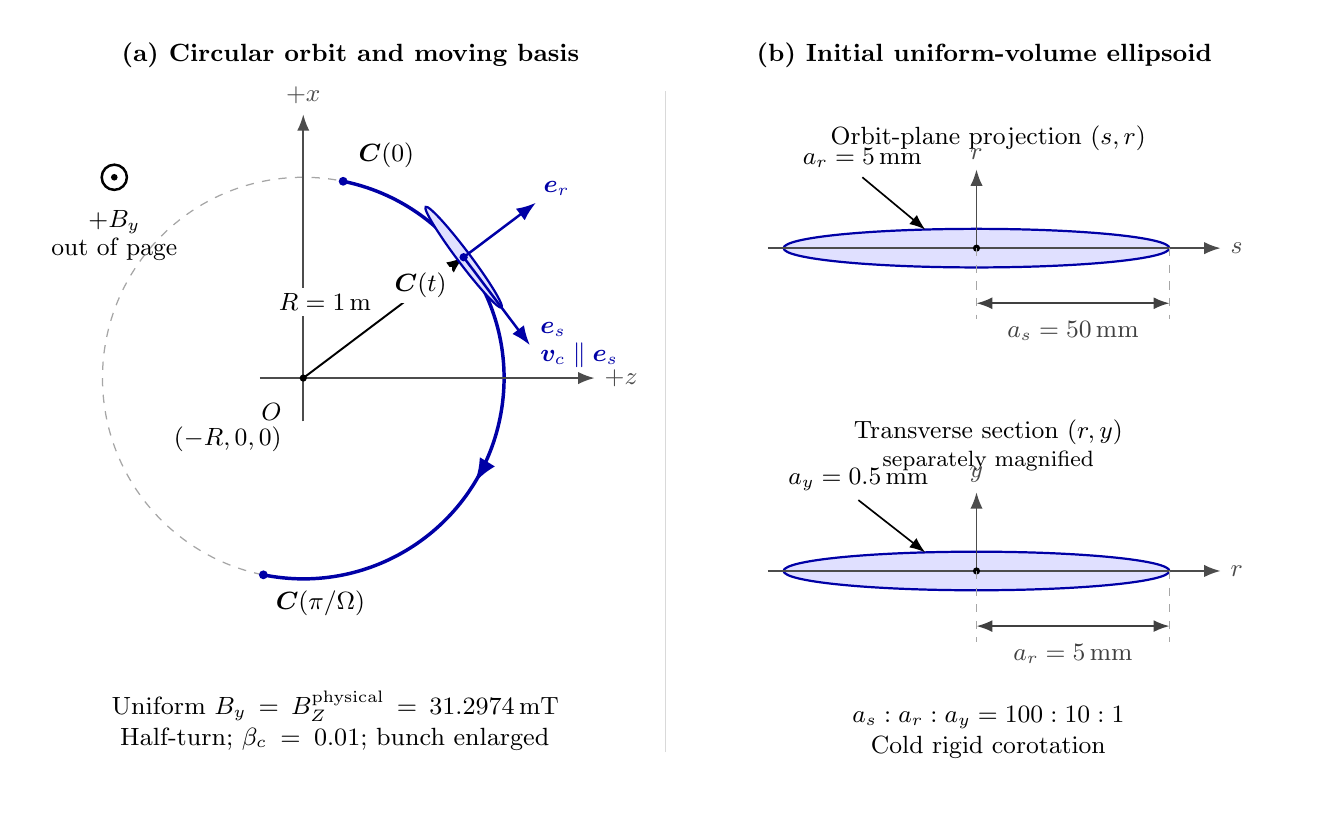
\begin{tikzpicture}[
  x=1cm,y=1cm,
  font=\small,
  >=Latex,
  axis/.style={->,line width=.65pt,black!70},
  dimension/.style={<->,line width=.6pt,black!75},
  localaxis/.style={->,line width=.9pt,blue!65!black},
  orbit/.style={line width=1.25pt,blue!65!black},
  guide/.style={line width=.45pt,dashed,black!35},
  bunch/.style={draw=blue!65!black,fill=blue!12,line width=.8pt},
  labelbox/.style={fill=white,inner sep=2pt}
 ]
 \path[use as bounding box] (0,0.55) rectangle (16.3,10.25);
 \node[font=\bfseries\small] at (4.1,9.9) {(a) Circular orbit and moving basis};
 \node[font=\bfseries\small] at (12.15,9.9) {(b) Initial uniform-volume ellipsoid};
 \draw[black!15] (8.1,1.05) -- (8.1,9.45);

 % Global laboratory orbit: (z,x+R) = (R sin(theta), R cos(theta)).
 \coordinate (O) at (3.5,5.8);
 \coordinate (C) at ($(O)+(37:2.55)$);
 \coordinate (Czero) at ($(O)+(78.540844:2.55)$);
 \coordinate (Cend) at ($(O)+(-101.459156:2.55)$);
 \draw[guide] (O) circle[radius=2.55];
 \draw[orbit,
   postaction={decorate},
   decoration={markings,mark=at position .61 with {\arrow{Latex}}}]
   (Czero) arc[start angle=78.540844,end angle=-101.459156,radius=2.55];
 \draw[axis] ($(O)+(-.55,0)$) -- ($(O)+(3.7,0)$) node[right] {$+z$};
 \draw[axis] ($(O)+(0,-.55)$) -- ($(O)+(0,3.35)$) node[above] {$+x$};
 \fill (O) circle[radius=1.3pt];
 \node[anchor=north east,align=right] at ($(O)+(-.15,-.2)$)
   {$O$\\[-2pt]$(-R,0,0)$};
 \draw[->,line width=.7pt] (O) -- (C)
   node[pos=.48,above left=1pt,labelbox] {$R=1\,\mathrm m$};

 % Tangentially long bunch; enlarged relative to the orbit.
 \begin{scope}[shift={(C)},rotate=-53]
   \draw[bunch] (0,0) ellipse[x radius=.8,y radius=.08];
 \end{scope}
 \fill[blue!65!black] (C) circle[radius=1.5pt];
 \node[labelbox,anchor=north east] at ($(C)+(-.14,-.12)$) {$\bm C(t)$};
 \draw[localaxis] (C) -- ($(C)+(37:1.15)$)
   node[above right=-1pt] {$\bm e_r$};
 \draw[localaxis] (C) -- ($(C)+(-53:1.4)$)
   node[right,align=left] {$\bm e_s$\\[-1pt]$\bm v_c\parallel\bm e_s$};
 \fill[blue!65!black] (Czero) circle[radius=1.6pt];
 \node[anchor=south west,labelbox] at ($(Czero)+(.12,.09)$)
   {$\bm C(0)$};
 \fill[blue!65!black] (Cend) circle[radius=1.6pt];
 \node[anchor=north west,labelbox] at ($(Cend)+(.08,-.13)$)
   {$\bm C(\pi/\Omega)$};

 % Field normal: positive y points toward the reader in this projection.
 \draw[line width=.9pt] (1.1,8.35) circle[radius=.16];
 \fill (1.1,8.35) circle[radius=.042];
 \node[anchor=north,align=center] at (1.1,8.05)
   {$+B_y$\\[-1pt]out of page};
 \node[align=center,text width=6.6cm,font=\small] at (3.9,1.45)
   {Uniform $B_y=B_Z^{\rm physical}=31.2974\,\mathrm{mT}$\\
    Half-turn; $\beta_c=0.01$; bunch enlarged};

 % Orbit-plane ellipsoid projection. Ratio a_s/a_r = 10 is preserved here.
 \node[align=center] at (12.2,8.85) {Orbit-plane projection $(s,r)$};
 \coordinate (P) at (12.05,7.45);
 \draw[bunch] (P) ellipse[x radius=2.45,y radius=.245];
 \draw[axis] ($(P)+(-2.65,0)$) -- ($(P)+(3.1,0)$) node[right] {$s$};
 \draw[axis] (P) -- ($(P)+(0,1.0)$) node[above] {$r$};
 \fill (P) circle[radius=1.3pt];
 \draw[guide] (P) -- ($(P)+(0,-.9)$);
 \draw[guide] ($(P)+(2.45,0)$) -- ($(P)+(2.45,-.9)$);
 \draw[dimension] ($(P)+(0,-.7)$) -- ($(P)+(2.45,-.7)$)
   node[midway,below=3pt] {$a_s=50\,\mathrm{mm}$};
 \draw[->,line width=.6pt] ($(P)+(-1.45,.9)$) -- ($(P)+(-.65,.235)$);
 \node[anchor=south,align=center] at ($(P)+(-1.45,.9)$)
   {$a_r=5\,\mathrm{mm}$};

 % Independently magnified thin cross-section. Ratio a_r/a_y = 10.
 \node[align=center] at (12.2,4.95)
   {Transverse section $(r,y)$\\[-1pt]\footnotesize separately magnified};
 \coordinate (S) at (12.05,3.35);
 \draw[bunch] (S) ellipse[x radius=2.45,y radius=.245];
 \draw[axis] ($(S)+(-2.65,0)$) -- ($(S)+(3.1,0)$) node[right] {$r$};
 \draw[axis] (S) -- ($(S)+(0,1.0)$) node[above] {$y$};
 \fill (S) circle[radius=1.3pt];
 \draw[guide] (S) -- ($(S)+(0,-.9)$);
 \draw[guide] ($(S)+(2.45,0)$) -- ($(S)+(2.45,-.9)$);
 \draw[dimension] ($(S)+(0,-.7)$) -- ($(S)+(2.45,-.7)$)
   node[midway,below=3pt] {$a_r=5\,\mathrm{mm}$};
 \draw[->,line width=.6pt] ($(S)+(-1.5,.9)$) -- ($(S)+(-.65,.235)$);
 \node[anchor=south,align=center] at ($(S)+(-1.5,.9)$)
   {$a_y=0.5\,\mathrm{mm}$};
 \node[font=\small,align=center] at (12.2,1.3)
   {$a_s:a_r:a_y=100:10:1$\\Cold rigid corotation};
\end{tikzpicture}

 \caption{Test geometry in OPALX coordinates. Left: the clockwise half-turn,
 radial and tangential axes, and $B_y$ out of the page (physical $B_Z$).
 The bunch is enlarged at an illustrative intermediate phase.
 Right: initial ellipsoid projections with separately magnified semiaxes.}
 \label{fig:test-geometry}
\end{figure}
The initial semiaxes satisfy $a_s:a_r:a_y=100:10:1$.
Particles start in rigid corotation with no random velocity spread.
The source has uniform volume density and finite thickness; it is not a uniform
areal disk.

\clearpage
\subsection{Affine ellipsoid model}
Dubin's reference gives the internal electrostatic field of a uniformly
charged three-dimensional ellipsoid. \Cref{fig:dubin-reference} separates
its geometry from the componentwise linear field law used in the affine
model. The illustration uses generic semiaxes; the numerical values remain
those specified for each test.
\begin{figure}[H]
 \centering
 % Dubin uniform-volume ellipsoid: schematic geometry, not new numerical data.
% Principal-axis coordinates are (u,y,s), with semiaxes (a_0,c_0,b).
% Different display scales are used for the three physical axes.
% No field-vector alignment with an arbitrary displacement is implied.
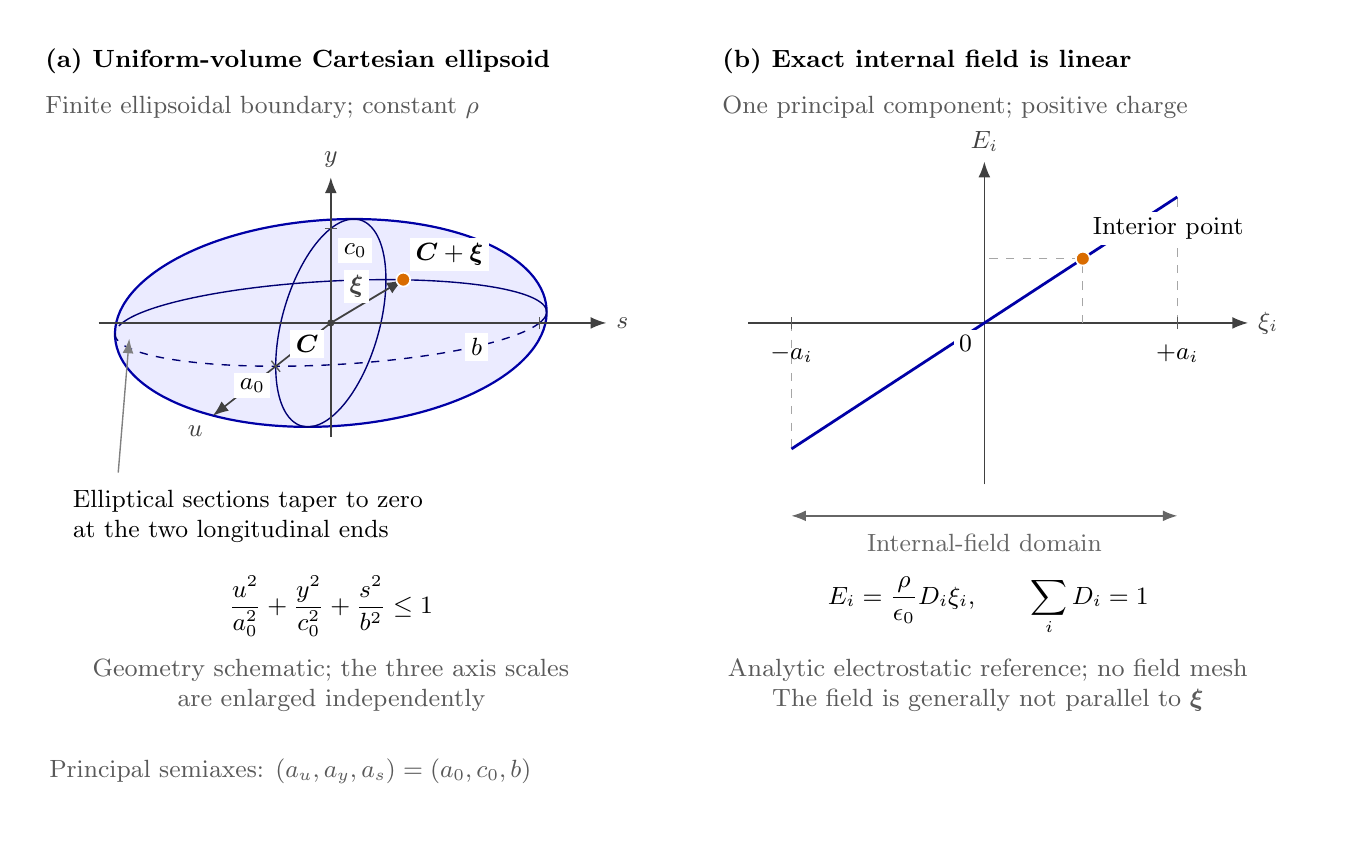
\begin{tikzpicture}[
 x=1cm,y=1cm,font=\small,>=Latex,
 duaxis/.style={->,black!75,line width=.6pt},
 dusource/.style={draw=blue!65!black,fill=blue!8,line width=.8pt},
 dusurface/.style={blue!45!black,line width=.5pt},
 duguide/.style={black!35,line width=.45pt,dashed},
 dulabel/.style={fill=white,inner sep=2pt},
 dutarget/.style={fill=orange!85!black,draw=white,line width=.6pt}
]
 \path[use as bounding box] (0,0) rectangle (16.6,10.0);
 \node[anchor=north west,font=\bfseries\small] at (.1,9.85)
   {(a) Uniform-volume Cartesian ellipsoid};
 \node[anchor=north west,font=\bfseries\small] at (8.7,9.85)
   {(b) Exact internal field is linear};
 \node[anchor=north west,black!65] at (.1,9.25)
   {Finite ellipsoidal boundary; constant $\rho$};
 \node[anchor=north west,black!65] at (8.7,9.25)
   {One principal component; positive charge};

 % Oblique projection of a triaxial ellipsoid. The three display-axis vectors
 % are S=(2.65,0), U=(-.7,-.55), Y=(0,1.2); the outer silhouette is their
 % projected ellipse, rounded to plotting precision. All display units are cm.
 \coordinate (duC) at (3.85,6.25);
 \begin{scope}[shift={(duC)},rotate=3.80]
   \draw[dusource] (0,0) ellipse[x radius=2.746,y radius=1.310];
 \end{scope}
 \begin{scope}[shift={(duC)}]
   \draw[dusurface,domain=0:180,samples=70,smooth,dashed]
     plot ({2.65*cos(\x)-.7*sin(\x)},{-.55*sin(\x)});
   \draw[dusurface,domain=180:360,samples=70,smooth]
     plot ({2.65*cos(\x)-.7*sin(\x)},{-.55*sin(\x)});
   \draw[dusurface,domain=0:360,samples=90,smooth]
     plot ({-.7*cos(\x)},{-.55*cos(\x)+1.2*sin(\x)});
 \end{scope}
 \draw[duaxis] ($(duC)+(-2.95,0)$) -- ($(duC)+(3.5,0)$)
   node[right] {$s$};
 \draw[duaxis] ($(duC)+(0,-1.45)$) -- ($(duC)+(0,1.85)$)
   node[above] {$y$};
 \draw[duaxis] (duC) -- ($(duC)+(-1.5,-1.18)$)
   node[below left] {$u$};
 \fill[black!75] (duC) circle[radius=1.3pt];
 \node[anchor=north east,dulabel] at ($(duC)+(-.08,-.08)$) {$\bm C$};

 % Semiaxis labels mark the three principal directions, rather than the
 % semiaxes of the projected outer silhouette.
 \draw[black!65,line width=.5pt] ($(duC)+(2.65,-.08)$) -- ($(duC)+(2.65,.08)$);
 \node[dulabel,anchor=north] at ($(duC)+(1.85,-.12)$) {$b$};
 \draw[black!65,line width=.5pt] ($(duC)+(-.08,1.2)$) -- ($(duC)+(.08,1.2)$);
 \node[dulabel,anchor=west] at ($(duC)+(.09,.92)$) {$c_0$};
 \draw[black!65,line width=.5pt] ($(duC)+(-.755,-.48)$) -- ($(duC)+(-.645,-.62)$);
 \node[dulabel,anchor=north east] at ($(duC)+(-.76,-.63)$) {$a_0$};

 % Interior material point. Only displacement is drawn; anisotropic D does
 % not generally give E parallel to xi.
 \coordinate (duP) at ($(duC)+(.92,.55)$);
 \draw[->,black!75,line width=.65pt] (duC) -- (duP)
   node[midway,above left=-1pt,dulabel] {$\bm\xi$};
 \fill[dutarget] (duP) circle[radius=2.5pt];
 \node[anchor=south west,dulabel] at ($(duP)+(.08,.1)$) {$\bm C+\bm\xi$};
 \node[anchor=north west,align=left] at (.45,4.25)
   {Elliptical sections taper to zero\\at the two longitudinal ends};
 \draw[black!50,line width=.5pt,->] (1.15,4.35) -- ($(duC)+(-2.56,-.2)$);

 % Schematic component plot. No numerical field values, slope fit or sampled
 % simulation data enter this graphic. It is the exact interior relation.
 \coordinate (duO) at (12.15,6.25);
 \draw[duaxis] ($(duO)+(-3.0,0)$) -- ($(duO)+(3.35,0)$)
   node[right] {$\xi_i$};
 \draw[duaxis] ($(duO)+(0,-2.05)$) -- ($(duO)+(0,2.05)$)
   node[above] {$E_i$};
 \foreach \sign in {-1,1} {
   \draw[duguide] ($(duO)+(\sign*2.45,0)$) -- ($(duO)+(\sign*2.45,\sign*1.6)$);
   \draw[black!65,line width=.5pt] ($(duO)+(\sign*2.45,-.08)$) -- ($(duO)+(\sign*2.45,.08)$);
 }
 \draw[blue!65!black,line width=1.0pt]
   ($(duO)+(-2.45,-1.6)$) -- ($(duO)+(2.45,1.6)$);
 \node[anchor=north] at ($(duO)+(-2.45,-.15)$) {$-a_i$};
 \node[anchor=north] at ($(duO)+(2.45,-.15)$) {$+a_i$};
 \node[anchor=north east,dulabel] at ($(duO)+(-.08,-.08)$) {$0$};
 \draw[duguide] ($(duO)+(1.25,0)$) -- ($(duO)+(1.25,.8163)$)
   -- ($(duO)+(0,.8163)$);
 \fill[dutarget] ($(duO)+(1.25,.8163)$) circle[radius=2.5pt];
 \node[anchor=south west,dulabel] at ($(duO)+(1.3,.98)$)
   {Interior point};
 \draw[<->,black!60,line width=.5pt]
   ($(duO)+(-2.45,-2.45)$) -- ($(duO)+(2.45,-2.45)$)
   node[midway,below=3pt] {Internal-field domain};

 \node[align=center] at (3.85,2.65)
   {$\displaystyle\frac{u^2}{a_0^2}+\frac{y^2}{c_0^2}+\frac{s^2}{b^2}\le1$};
 \node[align=center] at (12.2,2.65)
   {$\displaystyle E_i=\frac{\rho}{\epsilon_0}D_i\xi_i,\qquad \sum_iD_i=1$};
 \node[align=center,text width=7.5cm,black!65] at (3.85,1.65)
   {Geometry schematic; the three axis scales\\are enlarged independently};
 \node[align=center,text width=7.5cm,black!65] at (12.2,1.65)
   {Analytic electrostatic reference; no field mesh\\The field is generally not parallel to $\bm\xi$};
 \node[anchor=west,black!65] at (.15,.55)
   {Principal semiaxes: $(a_u,a_y,a_s)=(a_0,c_0,b)$};
\end{tikzpicture}

 \caption{Uniform-density ellipsoid in its principal-axis frame, with
 semiaxes $a_0,b,c_0$. Each internal field component is linear in its own
 coordinate. The field is generally not parallel to the displacement from
 the centre because the three depolarization factors differ. Geometry and
 component-field lines are schematic, not additional numerical results.}
 \label{fig:dubin-reference}
\end{figure}
The exact linear field applies inside an ellipsoid, including its finite
tapered ends. It does not give the exact field of a constant-section cylinder
or a finite-radius curved tube. The tapered SACR family in \cref{sec:sacr}
recovers this ellipsoid as its radius tends to infinity.

\clearpage
For $\bm u$ uniform in the unit ball, the position, density and covariance are
\begin{equation}
 \bm r=\bm C+A\bm u,\qquad
 \rho=\frac{3Q}{4\pi\det A},\qquad
 \Sigma=\frac15 AA^\T .\label{eq:affine}
\end{equation}
The internal electrostatic field is linear. For
$AA^\T=U\operatorname{diag}(a_1^2,a_2^2,a_3^2)U^\T$, it is
\begin{equation}
 \bm E=\frac{\rho}{\eps}D(\bm r-\bm C),\qquad
 D=U\operatorname{diag}(D_i)U^\T,\qquad
 D_i=\frac{a_1a_2a_3}{3}R_D(a_j^2,a_k^2,a_i^2),\quad \sum_iD_i=1,
 \label{eq:field}
\end{equation}
where $R_D$ is Carlson's elliptic integral and $(i,j,k)$ is cyclic.
With no electrostatic trap, the cold-fluid equations~\cite{dubin} reduce to
\begin{equation}
 J=\begin{pmatrix}0&1&0\\-1&0&0\\0&0&0\end{pmatrix},\qquad
 \Omega=\frac{qB_Z}{m},\qquad
 \ddot{\bm C}=\Omega J\dot{\bm C},\qquad
 \ddot A=\frac{q\rho}{m\eps}DA+\Omega J\dot A .\label{eq:model}
\end{equation}
The unrotated initial conditions are
\begin{equation}
 A_0=\operatorname{diag}(5,50,0.5)~\mathrm{mm},\quad
 \dot A_0=\Omega JA_0,\quad
 \bm C_0=(R,0,0)^\T,\quad
 \dot{\bm C}_0=(0,-\Omega R,0)^\T .
\end{equation}
At zero self-charge, the ellipsoid rotates rigidly with constant orbit-basis
sizes. The model is electrostatic and nonrelativistic; it neglects magnetic
self-fields, conducting boundaries, collisions and radiation. At $\beta\simeq
0.01$ the omitted relativistic terms are small. The affine solution remains
valid while $\det A>0$. No field data or fitted parameter enters the reference.

\subsection{Projection and acceptance}
The comparison projects the model covariance onto the recorded OPALX reference
axes $\bm e_i$. With $R_0=\exp(0.2J)$, this gives
\begin{equation}
 \Sigma_{\rm O}=T R_0AA^\T R_0^\T T^\T/5,\qquad
 \sigma_i^{\rm model}=\sqrt{\bm e_i^\T\Sigma_{\rm O}\bm e_i},\quad i\in\{r,s,y\}.
 \label{eq:projection}
\end{equation}
Independent model checks and their numerical errors are in
\cref{app:verification}.

\section{Numerical setup and error measures}
The archived tracking implementation uses longitudinal CIC and $g=6.36$.
The path and constant field map contain the full bunch and deposition support.
No additional curvature operator is used. Implementation and software checks
are in \cref{app:verification}.

The total-size error is
\begin{equation}
 \epsilon_i=\max_{t\in\mathrm{STAT}}
 \left|\frac{\sigma_i^{\rm OPALX}(t)}{\sigma_i^{\rm model}(t)}-1\right|.
 \label{eq:error}
\end{equation}
Acceptance requires $\epsilon_i<1\%$ in all directions, full duration, and
correct particle count and charge. Each independent refinement must change
all RMS curves by at most 0.5\% and remain within 1\% of the model.

Collective growth subtracts a matched self-field-off control:
\begin{equation}
 \Delta\sigma_i=\sigma_i(Q)-\sigma_i(\mathrm{SC\ off}),\qquad
 e_{\Delta,i}=\Delta\sigma_i^{\rm OPALX}-\Delta\sigma_i^{\rm model}.
 \label{eq:growth}
\end{equation}
Its relative error uses the model increase; absolute errors are used near zero.
For covariance, the standardized error is
\begin{equation}
 e_{ij}^{\Sigma}=\frac{\Sigma_{ij}^{\rm OPALX}-\Sigma_{ij}^{\rm model}}
 {\sigma_i^{\rm model}\sigma_j^{\rm model}}.\label{eq:covmetric}
\end{equation}
The self-field-off control retains 0.1 pC assigned charge for finite
macroparticle $q/m$, but uses zero model self-charge and the NONE solver.

\clearpage
\section{Baseline intensity scan}
\tabfile{baseline}
\reportfigure{baseline-rms}{Total RMS sizes and signed errors at every STAT
sample. Dashed: independent model; solid: OPALX. All four cases satisfy the
1\% total-size criterion.}{fig:baseline}
All runs complete the half-turn and retain 98,304 particles and assigned charge.
The largest error is 0.90323\%, radial at 1 pC. Collective-growth accuracy is
assessed separately below.

\clearpage
\section{Numerical refinements and 3D controls}
\subsection{Independent 1 pC FFT2D5 refinements}
\tabfile{convergence}
\reportfigure{baseline-refinement}{Maximum RMS changes from the baseline in
four independent full-half-turn refinements. The largest change is 0.31101\%;
all refined curves remain within 1\% of the model.}{fig:convergence}
The largest refined model error is 0.98585\%. These are separate one-parameter
controls, not a joint asymptotic extrapolation.

\subsection{3D OPEN control}
The same source and field are tracked with 3D OPEN on
$32\times32\times64$ and, for the refined 1 pC case, $64\times64\times128$
meshes. Charged cases use 128 steps; the charge-off row uses 512.
\tabfile{open}
At 1 pC, halving the step changes RMS sizes by at most 0.00831\%; doubling
particles changes them by 0.02515\%. One-/two-rank OPEN curves agree within
$3.5\times10^{-13}$ relative. This does not test distributed FFT2D5.

\clearpage
\section{Tenfold-charge stress test}
The 10 pC study uses a $40\times64$ mm FFT2D5 box. Coarse and fine meshes are
$128\times512\times1024$ and $256\times1024\times1024$, both with 128 steps.
The 3D OPEN control uses $64\times64\times128$ and 256 steps. All five runs,
including matched self-field-off controls, use one pinned executable.
\tabfile{strong}
\reportfigure{strong-charge-rms}{Completed 10 pC comparison with the independent
model (black dashed). Fine FFT2D5 retains large radial and tangential errors;
3D OPEN agrees within 0.070\% in every direction. Residuals use each run's
recorded reference axes.}{fig:strong}
All runs complete their promised duration and preserve particle count and
charge. All 80 saved snapshots stay inside the field map; both FFT cases also
clear the fixed box and outer CIC half-cell.
\tabfile{strongrefinement}
The transverse refinement changes radial and tangential sizes little, but the
1.92\% vertical change exceeds the 0.5\% convergence criterion. Longitudinal
resolution is unchanged. The final model extent ratio of about 2.14 also
stresses the long-bunch approximation; these results do not isolate $g$ as the
sole cause of the FFT2D5 discrepancy.

\clearpage
\section{Collective growth, covariance and centroid}
\subsection{Final increase from the matched control}
\textbf{1 pC:}\tabfile{growth1}
\textbf{Completed 10 pC controls:}\tabfile{growth10}
Tangential growth is 32.36\% high at 1 pC despite only 0.3838\% total-size
error. At 10 pC, fine FFT2D5 growth is 30.65\% high radially and 56.91\% high
tangentially; final OPEN growth errors remain below 0.14\%.
\reportfigure{collective-growth}{Completed 10 pC RMS increases from matched
self-field-off controls. Black dashed: independent model. Lower panels show
signed absolute growth errors for coarse/fine FFT2D5 and 3D OPEN.}{fig:growth}

\clearpage
\subsection{Covariance and centroid}
\tabfile{response}
The table gives the maximum centroid displacement from the matched control,
the final standardized covariance error against the model, and
radial--tangential correlation $\rho_{rs}$.
\reportfigure{centroid-covariance}{Charged-minus-control centroid displacement
and covariance error. The model predicts zero centroid response.
The 1 pC row is the archived baseline; the two 10 pC rows use the completed
study. Covariance uses one final 1 pC snapshot and 16 snapshots per 10 pC run.}{fig:response}

\clearpage
\section{Self-fields and the longitudinal model}
Initial self-fields are compared with the exact ellipsoid field. The
all-particle moment ratio and pointwise error are
\begin{equation}
 M_i=\frac{\sum_p\xi_{p,i}E_{p,i}^{\rm OPALX}}
 {\sum_p\xi_{p,i}E_{p,i}^{\rm exact}},\qquad
 L_i=\sqrt{\frac{\sum_p(E_{p,i}^{\rm OPALX}-E_{p,i}^{\rm exact})^2}
 {\sum_p(E_{p,i}^{\rm exact})^2}},
\end{equation}
where $\bm\xi_p$ is displacement from the centroid.
\tabfile{fields}
\reportfigure{initial-fields}{Initial all-particle field moments and pointwise
errors. Historical: $64\times128\times1024$, binary \code{415fff3b41df};
current: $128\times256\times2048$, binary \code{ba08fdd0b0bb}.
Both mesh and executable change; this is not a controlled convergence pair.}{fig:fields}
The current longitudinal moment is 21.281\% high. Pointwise longitudinal
force convergence is not established.

\clearpage
\subsection{Shape-dependent longitudinal equivalent}
For the initial semiaxes $(a,b,c)$, the exact longitudinal coefficient gives
$g_{\rm eq}=2b^2D_s/(ac)=5.223213$, compared with fixed $g=6.36$.
For a tilted ellipsoid, the moment equivalent is
\begin{equation}
 b_{\rm marg}=\sqrt{5\Sigma_{ss}},\qquad
 g_{\rm eq}=\frac{2b_{\rm marg}^3}{\det A}
 \frac{(D\Sigma)_{ss}}{\Sigma_{ss}},
\end{equation}
with $D$ and $\Sigma$ in the same ideal-centroid orbit basis.
\reportfigure{longitudinal-model}{Model-derived longitudinal moment equivalent
versus fixed $g=6.36$. It falls to 3.85049 at 1 pC and 1.90716 at 10 pC.
This diagnostic does not replace the full field tensor.}{fig:gmodel}
The initial mean radial self-field is $-0.3432$ V/m rather than zero;
99.5\% comes from the longitudinal projection in a circular-basis decomposition.

\clearpage
\section{Radius similarity scan}
Hold the source shape and centroid $\beta$ fixed and scale
\begin{equation}
 B=B_1\frac{1\,\mathrm m}{R},\qquad
 Q=Q_1\left(\frac{1\,\mathrm m}{R}\right)^2,\qquad
 t=t_1\frac{R}{1\,\mathrm m},\qquad Q_1=1~\mathrm{pC}.
\end{equation}
Since $Q/\Omega^2$ is constant, the model predicts identical sizes versus orbit
angle. Each radius uses regenerated corotation velocities, field map and path.
\tabfile{radius}
\reportfigure{radius-similarity}{Completed radius scan. Dashed: independent
model; solid: OPALX. All four cases satisfy the 1\% total-size criterion.
Residuals use each case's actual reference axes.}{fig:radius}
Physical mesh spacing is preserved; all saved snapshots clear the transverse
box and CIC edge. Instantaneous bunch spans are about
$2.9^\circ,5.7^\circ,11.5^\circ,22.7^\circ$ in descending radius order.
The $R=0.25$ m refinement remains incomplete.
Tangential-growth errors remain 32.34--32.88\%, while centroid shifts rise
from 6.67 to 53.52~$\mu$m. The longitudinal bias persists across radii;
curvature effects remain visible in the centroid.

\textbf{Conclusion.} Total RMS sizes meet 1\% in the tested baseline and radius
scan; collective growth does not. At 10 pC, OPEN agrees within 0.070\%, while
large in-plane FFT2D5 errors persist under transverse refinement. Complete the
tight-radius control and a same-executable initial-field study; vertical
strong-charge convergence remains open.

\clearpage
\section{Semi-analytic curved-tube reference (SACR)}
\label{sec:sacr}
SACR evaluates the free-space electrostatic field of a prescribed curved charge
distribution without a three-dimensional mesh. The target geometry is a 5 m
beam on a 2 m bend radius, spanning $143.24^\circ$, with 5 mm radial extent.
This section uses an ellipsoidally tapered source to obtain an exact Dubin
limit. \Cref{sec:frozen} extends the field comparison to a constant-section
tube; neither test establishes its self-consistent tracking accuracy.

\begin{figure}[H]
 \centering
 % Prescribed SACR sources and their distinct straight limits; no solver grid.
% The left envelope is u=+/-a0*sqrt(1-s^2/b^2), mapped onto a circular path.
% The midpoint source patch has a'=c'=0, so its outward normal is radial.
% Transverse dimensions are deliberately enlarged. Connections are geometry,
% not computed electric-field vectors or magnitudes.
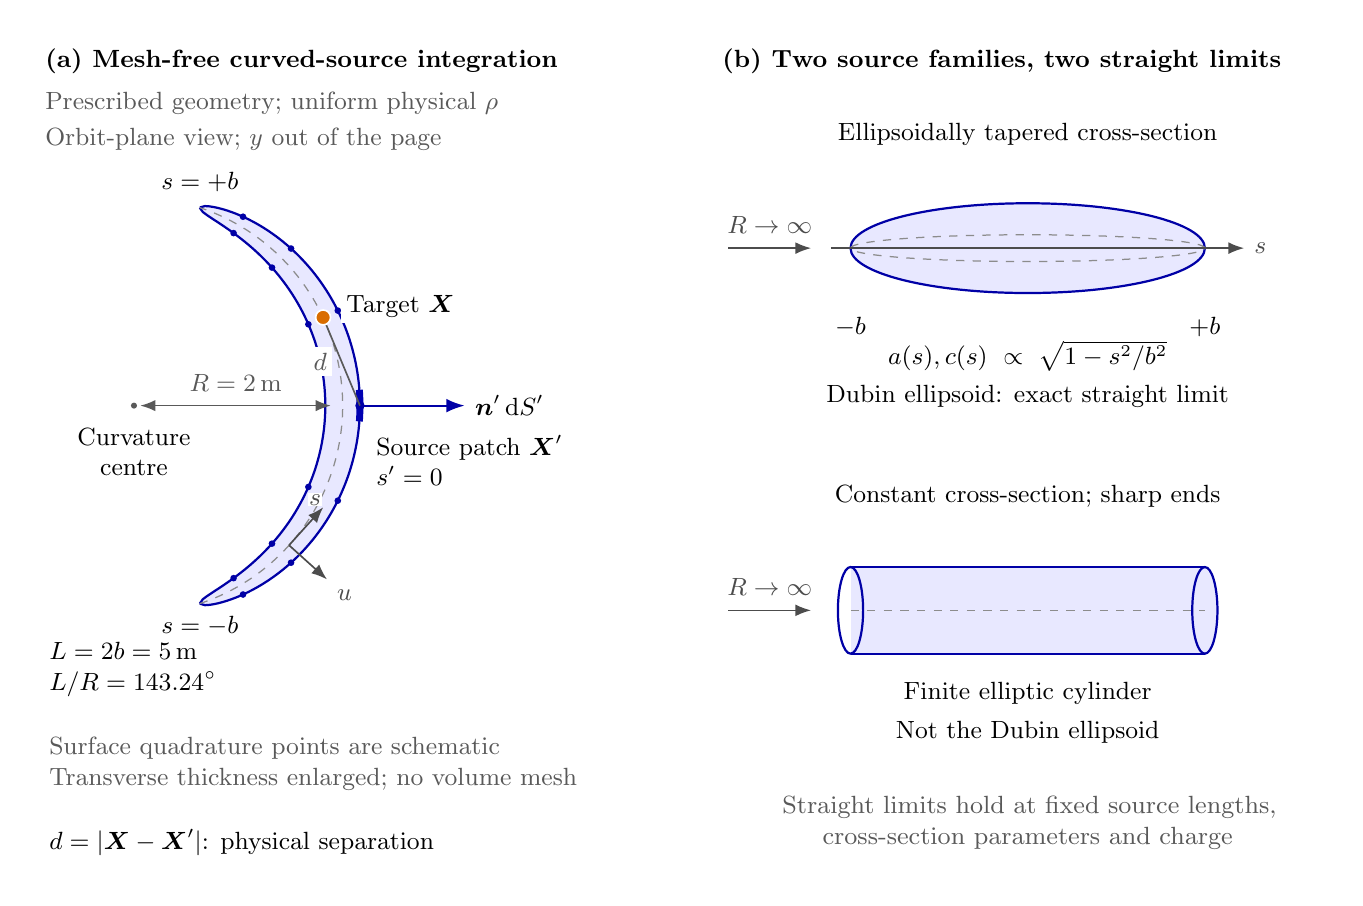
\begin{tikzpicture}[
 x=1cm,y=1cm,font=\small,>=Latex,
 srsource/.style={blue!65!black,line width=.8pt},
 srthin/.style={black!45,line width=.45pt},
 sraxis/.style={->,black!70,line width=.6pt},
 srdim/.style={<->,black!65,line width=.55pt},
 srlabel/.style={fill=white,inner sep=2pt},
 srtarget/.style={fill=orange!85!black,draw=white,line width=.6pt}
]
 \path[use as bounding box] (0,0) rectangle (16.6,10.8);
 \node[anchor=north west,font=\bfseries\small] at (.1,10.65)
   {(a) Mesh-free curved-source integration};
 \node[anchor=north west,black!65] at (.1,10.1)
   {Prescribed geometry; uniform physical $\rho$};
 \node[anchor=north west,black!65] at (.1,9.65)
   {Orbit-plane view; $y$ out of the page};
 \node[anchor=north west,font=\bfseries\small] at (8.7,10.65)
   {(b) Two source families, two straight limits};

 % Circular reference: 5 m source / 2 m radius = 143.239449 degrees.
 \coordinate (srO) at (1.35,6.0);
 \fill[blue!9]
  plot[domain=-71.619724:71.619724,samples=121]
   ({1.35+(2.65-.22*sqrt(max(0,1-(\x/71.619724)^2)))*cos(\x)},
    {6.0+(2.65-.22*sqrt(max(0,1-(\x/71.619724)^2)))*sin(\x)})
  -- plot[domain=71.619724:-71.619724,samples=121]
   ({1.35+(2.65+.22*sqrt(max(0,1-(\x/71.619724)^2)))*cos(\x)},
    {6.0+(2.65+.22*sqrt(max(0,1-(\x/71.619724)^2)))*sin(\x)}) -- cycle;
 \foreach \side in {-1,1} {
  \draw[srsource]
   plot[domain=-71.619724:71.619724,samples=121]
    ({1.35+(2.65+\side*.22*sqrt(max(0,1-(\x/71.619724)^2)))*cos(\x)},
     {6.0+(2.65+\side*.22*sqrt(max(0,1-(\x/71.619724)^2)))*sin(\x)});
 }
 \draw[srthin,dashed] ($(srO)+(-71.619724:2.65)$)
  arc[start angle=-71.619724,end angle=71.619724,radius=2.65];
 \foreach \theta in {-60,-45,-25,25,45,60} {
  \pgfmathsetmacro{\srwidth}{.22*sqrt(1-(\theta/71.619724)^2)}
  \fill[blue!65!black] ($(srO)+(\theta:{2.65+\srwidth})$) circle[radius=1.2pt];
  \fill[blue!65!black] ($(srO)+(\theta:{2.65-\srwidth})$) circle[radius=1.2pt];
 }

 % Source patch at the maximum cross-section: its normal is exactly radial.
 \coordinate (srP) at (4.22,6.0);
 \draw[blue!70!black,line width=2.5pt]
  plot[domain=-4:4,samples=15]
   ({1.35+(2.65+.22*sqrt(1-(\x/71.619724)^2))*cos(\x)},
    {6.0+(2.65+.22*sqrt(1-(\x/71.619724)^2))*sin(\x)});
 \fill[blue!65!black] (srP) circle[radius=1.7pt];
 \draw[->,blue!65!black,line width=.8pt] (srP) -- (5.55,6.0)
  node[right,black] {$\bm n'\,\dd S'$};
 \node[anchor=north west,srlabel,align=left] at (4.35,5.7)
  {Source patch $\bm X'$\\$s'=0$};
 \coordinate (srT) at ($(srO)+(25:2.65)$);
 \draw[black!65,line width=.6pt] (srP) -- (srT)
  node[midway,left=3pt,srlabel] {$d$};
 \fill[srtarget] (srT) circle[radius=2.7pt];
 \node[anchor=west,srlabel] at ($(srT)+(.22,.14)$)
  {Target $\bm X$};
 \draw[srdim] ($(srO)+(.08,0)$) -- (3.85,6.0)
  node[midway,above=3pt,srlabel] {$R=2\,\mathrm m$};
 \fill[black!65] (srO) circle[radius=1.1pt];
 \node[anchor=north,align=center] at ($(srO)+(0,-.16)$)
  {Curvature\\centre};
 \node[anchor=south,srlabel] at ($(srO)+(71.619724:2.65)+(0,.12)$)
  {$s=+b$};
 \node[anchor=north,srlabel] at ($(srO)+(-71.619724:2.65)+(0,-.08)$)
  {$s=-b$};

 % A local radial/tangential basis away from the integration target.
 \coordinate (srB) at ($(srO)+(-42:2.65)$);
 \draw[sraxis] (srB) -- ($(srB)+(-42:.65)$) node[below right] {$u$};
 \draw[sraxis] (srB) -- ($(srB)+(48:.65)$)
  node[above left,srlabel,inner sep=.5pt] {$s$};
 \node[anchor=west,align=left] at (.15,2.65)
  {$L=2b=5\,\mathrm m$\\$L/R=143.24^\circ$};
 \node[anchor=west,align=left,black!65] at (.15,1.45)
  {Surface quadrature points are schematic\\
   Transverse thickness enlarged; no volume mesh};
 \node[anchor=west] at (.15,.45)
  {$d=|\bm X-\bm X'|$: physical separation};

 % Family 1: fixed material semiaxes, curvature tends to zero.
 \node[align=center] at (12.7,9.45)
  {Ellipsoidally tapered cross-section};
 \draw[sraxis] (8.9,8.0) -- (9.95,8.0)
  node[midway,above=3pt,srlabel] {$R\to\infty$};
 \draw[srsource,fill=blue!9] (12.7,8.0) ellipse[x radius=2.25,y radius=.57];
 \draw[srthin,dashed] (12.7,8.0) ellipse[x radius=2.25,y radius=.17];
 \draw[sraxis] (10.2,8.0) -- (15.45,8.0) node[right] {$s$};
 \node[anchor=north] at (10.45,7.25) {$-b$};
 \node[anchor=north] at (14.95,7.25) {$+b$};
 \node[align=center] at (12.7,6.4)
  {$a(s),c(s)\ \propto\ \sqrt{1-s^2/b^2}$\\[3pt]
   Dubin ellipsoid: exact straight limit};

 % Family 2: the same limit does not turn a constant-section source into an ellipsoid.
 \node[align=center] at (12.7,4.85)
  {Constant cross-section; sharp ends};
 \draw[sraxis] (8.9,3.4) -- (9.95,3.4)
  node[midway,above=3pt,srlabel] {$R\to\infty$};
 \fill[blue!9] (10.45,2.85) rectangle (14.95,3.95);
 \draw[srsource] (10.45,2.85) -- (14.95,2.85);
 \draw[srsource] (10.45,3.95) -- (14.95,3.95);
 \draw[srsource] (10.45,3.4) ellipse[x radius=.16,y radius=.55];
 \draw[srsource,fill=blue!9] (14.95,3.4) ellipse[x radius=.16,y radius=.55];
 \draw[srthin,dashed] (10.45,3.4) -- (14.95,3.4);
 \node[align=center] at (12.7,2.1)
  {Finite elliptic cylinder\\[3pt]Not the Dubin ellipsoid};
 \node[align=center,black!65,text width=7.5cm] at (12.7,.7)
  {Straight limits hold at fixed source lengths,\\
   cross-section parameters and charge};
\end{tikzpicture}

 \caption{SACR is a mesh-free Coulomb reference for a prescribed physical
 charge distribution. Source-surface patches contribute through their
 outward vector areas and physical source-target separations. At fixed
 semiaxes and charge, $R\to\infty$ maps the ellipsoidally tapered family to
 Dubin's straight ellipsoid; a constant-section tube instead tends to a
 finite elliptic cylinder. Surface-only integration shown here assumes
 uniform physical density; a varying longitudinal density also requires
 the volume-gradient term. Transverse dimensions are enlarged.}
 \label{fig:sacr-reference-geometry}
\end{figure}
The finite-radius source is retained in the Coulomb distance. Its geometry
is integrated directly, without the IPPL grid or the first-order transverse
curvature expansion used by the OPALX OPEN backend. The two straight limits
in the illustration therefore describe different physical reference sources.
The reference-path coordinate map is orthogonal but not conformal: its scale
factors are $1,1,1+u/R$. The curved fields are evaluated from physical Coulomb
distances, rather than obtained by a conformal transformation of a straight
beam solution.
This describes the present method; it does not rule out other mapped
formulations, which must still represent the physical three-dimensional
source and its longitudinal coupling.

\clearpage
\subsection{Field model and straight limit}
For reference arclength $s$, outward radial displacement $u$ and vertical
coordinate $y$, the OPALX laboratory position and volume element are
\begin{align}
 \bm X(s,u,y)&=\big((R+u)\cos(s/R)-R,\ y,\ (R+u)\sin(s/R)\big)^\T,\\
 \dd V&=\left(1+\frac{u}{R}\right)\dd s\,\dd u\,\dd y.
 \label{eq:sacr-map}
\end{align}
For uniform physical volume density $\rho$, the Coulomb field has the exact
surface form
\begin{equation}
 \bm E(\bm x)=\frac{\rho}{4\pi\eps}
 \int_V\frac{\bm x-\bm x'}{|\bm x-\bm x'|^3}\,\dd V'
 =\frac{\rho}{4\pi\eps}
 \oint_{\partial V}\frac{\bm n'(\bm x')}{|\bm x-\bm x'|}\,\dd S'.
 \label{eq:sacr-surface}
\end{equation}
The second equality follows from the divergence theorem, with outward source
normal $\bm n'$. Two-dimensional boundary quadrature gives all three field
components, without a fitted $g$ or softening length.

For the Dubin comparison, choose
\begin{equation}
 a(s)=a_0\sqrt{1-s^2/b^2},\qquad
 c(s)=c_0\sqrt{1-s^2/b^2},\qquad |s|\le b,\qquad L=2b.
 \label{eq:sacr-taper}
\end{equation}
The physical density is constant, while the line density is parabolic.
The volume remains $4\pi a_0bc_0/3$ under bending: the term odd in $u$ in
\cref{eq:sacr-map} integrates to zero. At fixed semiaxes and charge,
$R\to\infty$ gives the Cartesian ellipsoid and its exact field
$E_i=\rho D_i x_i/\eps$ from Dubin~\cite{dubin}. Our $D_i$ equal half of
Dubin's coefficients, so $\sum_iD_i=1$.

A constant-section tube instead approaches a finite cylinder as $R\to\infty$;
it is not the finite ellipsoid used in this check. The 0.5 mm vertical semiaxis
in the thin verification cases is a benchmark choice, not a newly specified
real-beam parameter.

For an independent tangential check, let $A$ be the transverse ellipse
$u^2/a_0^2+y^2/c_0^2\le1$. At target $(u_t,y_t,s_t)$ define
$r_t=R+u_t$, $r_s=R+u$ and
$s_\pm=\pm b\sqrt{1-u^2/a_0^2-y^2/c_0^2}$. Exact integration along each
source filament gives
\begin{equation}
 E_s=\frac{\rho}{4\pi\eps}\int_A\frac{r_s}{r_t}
 \left(\frac{1}{d_+}-\frac{1}{d_-}\right)\dd u\,\dd y,
 \qquad d_\pm=|\bm X(s_t,u_t,y_t)-\bm X(s_\pm,u,y)|.
 \label{eq:sacr-endpoint}
\end{equation}
The straight limit has $r_s/r_t\to1$; the tapered source requires these
transverse-dependent ends.

\subsection{Error measures}
Fields are compared at matched material coordinates $\bm\xi=(u,y,s)$ and projected
onto each target's local radial, vertical and tangential basis. Let
$E_i^{\rm SACR}(R;\bm\xi)$ denote that local field and
$\ell_i=(a_0,c_0,b)_i$. Define
\begin{equation}
 E_{i,*}=\frac{\rho}{\eps}D_i\ell_i,\qquad
 \delta_i(R,\bm\xi)=\frac{E_i^{\rm SACR}(R;\bm\xi)-E_i^{\rm Dubin}(\bm\xi)}{E_{i,*}}.
 \label{eq:sacr-error}
\end{equation}
This component scale retains targets where the exact field vanishes. Changes
under quadrature refinement measure numerical resolution; finite-$R$
differences from Dubin also contain the physical curvature effect.

\clearpage
\subsection{Multi-point straight-limit checks}
The study uses 33 interior points per geometry: the centre, axis and midplane
points, signed off-axis points, and points near the ends and boundary. The
largest normalized ellipsoidal radius is 0.911. Three geometries are checked:
a 5 mm sphere, the previous $(5,50,0.5)$ mm ellipsoid, and a
$(5,2500,0.5)$ mm ellipsoid. Each value in the table is a maximum over all
33 points, expressed as a percentage of the corresponding component scale.
\tabfile{sacrflat}
\reportfigure{sacr-flat-limit}{Straight-limit SACR fields versus Dubin at all
33 points per geometry. The dashed identity line is the exact ellipsoid
field. Lower panels retain signed residuals, including zero-field targets;
normalization uses $E_{i,*}$ rather than the local field value.}{fig:sacr-flat}
Angular quadrature starts at 128 nodes and refines to at most 4096 where
needed. The largest measured straight-limit difference is
$3.97\times10^{-14}E_{i,*}$. The largest last-refinement change over the full
study is $3.64\times10^{-9}E_{i,*}$, below the requested $10^{-8}E_{i,*}$
criterion. These are sampled field checks, not a uniform error bound over the
entire charge distribution.
Dubin's coefficients set component scales and quadrature stopping criteria;
the fields themselves come from the Coulomb integral. A separate scalar
implementation agrees with the vectorized calculation within
$1.68\times10^{-14}E_{i,*}$.

\clearpage
\subsection{Radius convergence to Dubin}
For the 5 m tapered source, $a_0=5$ mm, $b=2.5$ m and $c_0=0.5$ mm are fixed
while $R$ varies from 2 to 2000 m and infinity. The same 33 material points
are used at each radius. The finite-radius difference contains the physical
change from a curved source to a straight ellipsoid; it is not an SACR error.
\reportfigure{sacr-radius-limit}{Convergence of the 5 m SACR source toward the
straight Dubin field. Solid curves show $\max_{\bm\xi}|\delta_i|$ over the 33
points; dashed curves show the separate last quadrature-refinement changes.
The $R=\infty$ checks are reported in the preceding table, not placed at an
artificial finite coordinate on this logarithmic axis.}{fig:sacr-radius}
\tabfile{sacrradius}
At $R=2$ m, the largest curvature differences are 0.3859\% radial,
0.4112\% tangential and 0.002801\% vertical, on the component scales defined
in \cref{eq:sacr-error}. All three decrease toward the straight limit. At
2000 m the vertical difference remains about 7.7 times the last-refinement
change; no universal $1/R^2$ rate is assumed.

An independent tangential endpoint integral agrees with the surface field
within $6.97\times10^{-15}E_{s,*}$ across 99 comparisons. Symmetry checks retain
the expected tangential/vertical zeros. At three interior points with $R=2$ m,
Cartesian finite differences use $\bm F=4\pi\eps\bm E/\rho$, whose exact
interior identities are $\nabla\cdot\bm F=4\pi$ and
$\nabla\times\bm F=\bm0$. The maximum errors are
$|\nabla\cdot\bm F/(4\pi)-1|=5.20\times10^{-12}$ and
$|\nabla\times\bm F|/(4\pi)=5.23\times10^{-12}$.
An independent volume integral at the bend centre, outside the source, agrees
with the boundary integral within $6.88\times10^{-13}$ relative.

This validates SACR's static field operator on the tested tapered family.
\Cref{sec:frozen} treats constant-section fields and their OPALX comparison.
A fixed prescribed tube does not supply a tracking reference after space
charge deforms its density.


\clearpage
\section{Historical frozen fields of a 5 m curved tube}
\label{sec:frozen}
Uniform physical density fills a sharp-ended tube with $L=5$ m, $R=2$ m and
radial/vertical semiaxes $a=5$ mm, $c=0.5$ mm. The nominal charge is 10 pC;
fields scale linearly. The vertical size and $\beta=0.001$ are benchmark
choices. One $10^{-17}$ s native step with zero external fields tests the
frozen field operator, not tracking. These results retain the earlier
independent-slice OPEN executable; \cref{sec:free-open} tests its replacement.

\subsection{Reference, native fields and comparison scales}
SACR uses \cref{eq:sacr-surface} and the same curved map, now with
$|s|\le L/2$ and $u^2/a^2+y^2/c^2\le1$. For $u=a\cos\phi$, $y=c\sin\phi$,
the side and cap vector areas are
\begin{align}
 \dd\bm A_{\rm side}&=(1+u/R)
  \big[c\cos\phi\,\bm e_r(s)+a\sin\phi\,\bm e_y\big]\dd s\,\dd\phi,\nonumber\\
 \dd\bm A_\pm&=\pm\bm e_s(\pm L/2)\dd u\,\dd y.
 \label{eq:frozen-area}
\end{align}
Thus $Q=\rho\pi acL$. Sampling includes the volume Jacobian $1+u/R$;
end caps do not. Independent endpoint, symmetry, divergence/curl, cylinder
and volume checks pass; the final SACR refinement change is below
$6.8\times10^{-12}$ of the component scales.

At 43 interior targets, native fields are transformed from the tracker frame
to the exact circle basis; a probe-only companion removes diagnostic charge.
Count, charge, IDs, finite-field and frame checks pass; probe motion is below
5 pm. The pinned executable is the completed 10 pC build in Appendix~B.

With $F_i=E_i/(\rho/(4\pi\eps))$, use fixed scales
\begin{equation}
 F_{r,*}=F_{y,*}=\frac{4\pi ac}{a+c},\qquad
 F_{s,*}=\max_{43\ {\rm targets}}|F_s^{\rm SACR}|,\qquad
 \eta_i=\frac{E_i^{\rm FFT2D5}-E_i^{\rm SACR}}{E_{i,*}}.
 \label{eq:frozen-scales}
\end{equation}
Here $E_{i,*}=\rho F_{i,*}/(4\pi\eps)$. These retain zeros; percentages are
not pointwise relative errors. At 10 pC the scales are 13.07 and 3.250 V/m.

\reportfigure{frozen-field-comparison}{All three fields at the 43 targets.
The finest member of each separate scan is shown, with no joint fine-mesh
run implied. Dashed: SACR identity. Lower panels retain signed differences.}{fig:frozen-fields}

\clearpage
\subsection{Separate mesh refinements and controls}
The transverse scan uses one quiet Cartesian cross-section source with
$N_y=N_x/2$ and fixed $N_z=512$; the longitudinal scan fixes
$N_x\times N_y=128\times64$.
Within each scan the source and reference path are held fixed.
\tabfile{frozenmeshes}
\reportfigure{frozen-mesh-convergence}{Matched-source refinements. Solid:
all 43 targets; dotted triangles: 31 targets at least 50 mm from either end.
Gray squares are successive mesh changes, separate from SACR difference.
The 1\% line uses the fixed component scale.}{fig:frozen-mesh}
\tabfile{frozenerrors}
``Interior'' includes the 50 mm end-distance targets; near-end targets lie
5 or 10 mm from an end. The 1\% all-component goal is not met. Stable
transverse refinement at fixed $N_z=512$ does not establish joint convergence
of the end fields or physical accuracy.

The last transverse mesh change is 0.00469\% radial and 0.0488\% vertical. Longitudinal source/path controls change $E_s$ by less than 0.000236\% of its scale, leaving the end-field failure unchanged.


At the reference-path midpoint $(u,y,s)=0$, not the global charge centroid,
the flat-slice continuum model with $\rho_{\rm slice}=\rho(1+u/R)$ predicts
\begin{equation}
 E_r^{\rm slice}(0)=-\frac{\rho}{2\pi\eps R}
 \int_A\frac{u^2}{u^2+y^2}\dd u\,\dd y
 =-\frac{\rho a^2c}{2\eps R(a+c)}
 =-0.016341\ {\rm V/m}\quad(10\ {\rm pC}).
 \label{eq:frozen-flat-slice}
\end{equation}
This unfitted slice prediction is inward; the full curved-tube field is outward.

\clearpage
\subsection{End response and the curvature field}
\reportfigure{frozen-native-longitudinal-end}{Native longitudinal fields on
a fixed transverse source column, $u=-42.98\,\mu$m, $y=-88.28\,\mu$m.
SACR and FFT2D5 use the same local polyline direction. Fields are rescaled
to exactly 10 pC. The dense SACR curve is a checked interpolant; the
43-target error metrics use direct quadrature.}{fig:frozen-end}
At 5 mm from an end, the finest longitudinal mesh misses essentially the
entire finite-tube tangential field. The local line-density-gradient model
does not reproduce the smooth interior end response of the Coulomb integral.

\reportfigure{frozen-centre-radial}{Centre radial field under the matched
transverse refinement. Black: full SACR curved-tube field; the second
analytic line is the flat-slice limit in \cref{eq:frozen-flat-slice}.
The FFT2D5 response has the opposite sign to SACR.}{fig:frozen-centre}
The finest transverse run gives $E_r(0)=-0.017629$ V/m, whereas SACR gives $+0.055092$ V/m: a 132.0\% difference relative to the centre field itself. 

One percent of the transverse scale is 0.131 V/m, larger than the entire
SACR centre field. Component-scale agreement cannot certify this response.
The archived field model fails this test. \Cref{sec:free-open} tests its
replacement; curved tracking remains unvalidated.

\clearpage
\section{Literature context and interpretation}
\label{sec:literature}
The archived frozen test identifies limits of the earlier FFT2D5 closures for a
specified source and observable. It does not show that all 2.5D methods fail.
Numerical convergence, physical-model accuracy and tracking accuracy remain
separate questions.

\subsection{The longitudinal closure matters}
The label 2.5D does not specify a unique solver. For example, ImpactX
distinguishes line-density-weighted transverse fields with a density-derivative
longitudinal kick from its Gaussian potential-based model and full 3D
models~\cite{impactx}. The archived OPALX operator solves separate transverse slices and adds
the open-space local closure
\begin{equation}
 E_s^{\rm local}(s)=-\frac{g_0}{4\pi\eps\gamma^2}
 \frac{\dd\lambda}{\dd s},\qquad g_0=6.36.
 \label{eq:literature-local}
\end{equation}
The value and formula are verified in the tested source code. For the
constant-section source, $\lambda$ is constant inside its sharp ends.
Therefore no finite choice of $g_0$ can recover a nonzero interior end field
where $\lambda'=0$. Refinement can resolve the density step more sharply
without recovering the finite-width Coulomb response in \cref{fig:frozen-end}.
This is our closure-level inference, independent of numerical end padding.

de Hoon et al.'s author manuscript derives a nonlocal Fourier--Bessel field and recovers the local
$g$ approximation by Taylor expansion; they explicitly identify end-region
breakdown~\cite{dehoon}. Their field is transversely averaged for a straight,
circularized beam in a conducting circular pipe. It supports the scope
diagnosis, not a quantitative prediction for our open elliptical arc; their
$R$ denotes pipe radius, not bending radius.

Oeftiger and Hegglin's equivalent longitudinal model uses a parabolic line
density; their Figure 1 gives $g_0=6.36$ for one free-space example. Their
$z_m>3r_p$ pipe-validity condition concerns a round conducting pipe,
not our free-space source~\cite{oeftiger}.
Oeftiger's thesis makes the ellipsoid's free-space $g_0$ shape-dependent~\cite{oeftigerthesis}.
Thus the matching code constant is a provenance clue, not a universal value
or proof of the original developer's intent.

Baartman distinguishes on-axis from transversely averaged forces in a round
grounded pipe; even their additive constants differ~\cite{baartman}.
Pipe, open-space, averaging and transverse-profile conventions must therefore
be matched before comparing numerical $g$ values.

Venturini and Wang--Li retain wavelength-dependent longitudinal response
rather than one constant~\cite{venturini,wangli}. Wang--Li include a 20 keV
$\mathrm H_2^+$ case with $\beta\simeq0.0046$ and 5 mm radius, but for a
straight round beam. These kernels motivate a nonlocal longitudinal model; they are not
already references for our finite curved ellipse.

\clearpage
\subsection{Curvature and validation scope}
For our geometry, the local metric and total-angle measures are different:
\begin{equation}
 \frac{a}{R}=0.0025,\qquad \frac{L}{R}=2.5\ {\rm rad},\qquad
 \frac{\gamma\sigma_s}{\sigma_r}\simeq577,
 \quad \sigma_s=\frac{L}{\sqrt{12}},\quad\sigma_r\simeq\frac a2.
 \label{eq:literature-geometry}
\end{equation}
Small $a/R$ is consistent with a local weak-curvature expansion. The
$143.24^\circ$ span does not by itself invalidate it, while global Cartesian
slicing would misrepresent the arc. The RMS aspect ratio uses the radial
width consistently; the still larger ratio based on the thin vertical width
does not remove the radial or end-field question.

Qiang's 2025 solver derives all kicks from one potential and treats curvature
perturbatively for smooth long bunches. Its Gaussian aspect-ratio illustration
above 1000 is not a strict 1\% validity bound~\cite{qiang2025}.
The improved 2026 preprint adds free-space reference-radius matching in
Eqs. 48--54~\cite{qiang2026}; that material must not be attributed to the
published 2025 version.

The 2026 regularized Gaussian curvature potential adds a linear term to
remove an integral divergence. Its displayed correction has zero on-axis
radial derivative as written~\cite{qiang2026}; this derivative statement is
our inference. It therefore does not directly predict our finite-arc centre
field of $+0.055092$ V/m. Comparison requires matching the global physical
source, boundary conditions and reference-force convention, which is distinct
from numerical mesh padding. No intent to remove a reference force is inferred.

Zhou et al.'s HB2025 study shows why long-arc frame reconstruction must be
checked independently of the field closure~\cite{zhou2025}.
The accepted 2026 paper describes a dynamic orbit-based frame, but only its
abstract was accessible; no radius-specific error bound can be extracted
from it~\cite{zhou2026}. Our frame controls address this numerical concern;
they do not supply the missing nonlocal end or curvature field.

Validation observables also differ. ImpactX's Gaussian single-kick example
tests a reduced-model kick against the same model's analytic prediction;
its acceptance tolerances are not a universal 1\% physical guarantee~\cite{impactx}.
SACR instead supplies an independent Coulomb reference for our prescribed
physical density. The sign error at the reference-path midpoint and the
5 mm end-field deficit limit the accuracy claim for the archived closure in
this stress case. They neither invalidate smooth-bunch applications nor
establish tracking errors.

Our 43-target metrics use raw laboratory electric fields. A charge-weighted
transverse average for the curved source would instead be
\begin{equation}
 \overline E_s(s)=\frac{\int_A\rho J E_s\,\dd u\,\dd y}
 {\int_A\rho J\,\dd u\,\dd y},\qquad J=1+u/R.
 \label{eq:literature-average}
\end{equation}
This average has not been computed; the 43 diagnostic points are not a
charge-weighted quadrature.

These findings motivated the nonuniform-density SACR extension and nonlocal
OPEN operator in \cref{sec:free-open}. Its triangular reference uses a weighted
boundary plus density-gradient volume term, rather than the earlier uniform
boundary-only identity. The new test compares the same finite physical source
with its full Coulomb field. Varying-curvature paths, retarded fields and
self-consistent curved tracking remain separate validation questions.

\clearpage
\section{Triangular bunch in a conducting circular pipe}
\label{sec:triangle-pipe}
This control reproduces the longitudinal-force component of the straight
round-pipe triangular-profile benchmark used in ORBIT~\cite{orbit2006,pyorbit3triangle}.
The new explicit \code{CIRCULAR_UNIFORM} model is compared with the
analytic solution, the earlier \code{CIRCULAR} model and repeated PyORBIT
calculations. This is a frozen-field test, not a tune-shift or tracking test.

The source has fixed circular radius $a=5$ mm, full length $L=10$ m,
$N=10^{14}$ protons and kinetic energy $0.4$ GeV. The grounded pipe radius
is $b=20$ mm. With $s=0$ at the bunch centre,
\begin{align}
 \lambda(s)&=\frac{2Q}{L}\left(1-\frac{2|s|}{L}\right),\quad |s|<L/2,
 & E_s(r,s)&=-\frac{\lambda'(s)}{4\pi\eps\gamma^2}\,g(r),\label{eq:triangle-pipe}\\
 g(r)&=\begin{cases}
 1+2\ln(b/a)-r^2/a^2,&0\le r\le a,\\
 2\ln(b/r),&a<r\le b.
 \end{cases}
 \label{eq:triangle-pointwise-g}
\end{align}
The density vanishes outside its support. On axis, $g=3.772589$ and
$E_*=|E_s|=10.681199$ kV/m; its uniform-disk average is
$\overline g=1/2+2\ln(b/a)$~\cite{baartman}.
Acceptance uses the same 62 on-axis and 82 radial targets at
$1\le|s|\le4$ m, excluding the cusp and ends. No coefficient is fitted.
A proton's equivalent one-metre kick is $\Delta W[\mathrm{eV}]=E_s[\mathrm{V/m}]$.

\reportfigure{triangle-pipe-fixed-fields}{Frozen on-axis fields and signed
difference from the physical analytic solution (black dashed). Gray crosses
retain the pre-change CIRCULAR result; blue circles use CIRCULAR\_UNIFORM.
PyORBIT variants are rerun independently. Residuals use the fixed scale
$E_*$; gray regions are excluded and the gray band marks $\pm1\%$.
The displayed cusp transition has no accuracy claim.}{fig:triangle-pipe-fixed-fields}
\tabfile{triangle-fixed-results}
Both columns are maximum pointwise relative physical field errors; accepted
reference values are nonzero. The fine new OPALX model meets 1\% on both
target sets. Its maximum differences from PyORBIT slices and Baartman
are 0.447\% and 0.167\%, respectively, relative to the local analytic field.

\clearpage
\subsection{Separate physical geometry from the numerical mesh}
The pointwise model requires explicit \code{PIPERADIUS}$=b\ge a$ and
\code{BEAMR}$=a$. \code{PIPESIZEX/Y} specify full open numerical widths
$W_x,W_y$. The physical radius is independent of these widths.
\begin{figure}[H]
\centering
\begin{minipage}[c]{0.53\linewidth}
\small
Model-specific settings for this benchmark:
\begin{verbatim}
FS: FIELDSOLVER, TYPE="FFT2D5",
 PIPEMODE="CIRCULAR_UNIFORM",
 BEAMR=0.005, PIPERADIUS=0.020,
 PIPESIZEX=0.020, PIPESIZEY=0.020,
 NX=128, NY=128, NZ=128,
 PARFFTX=FALSE, PARFFTY=FALSE,
 PARFFTZ=FALSE,
 REFPATHFNAME="straight-path.dat";
\end{verbatim}
\end{minipage}\hfill
\begin{minipage}[c]{0.44\linewidth}
\centering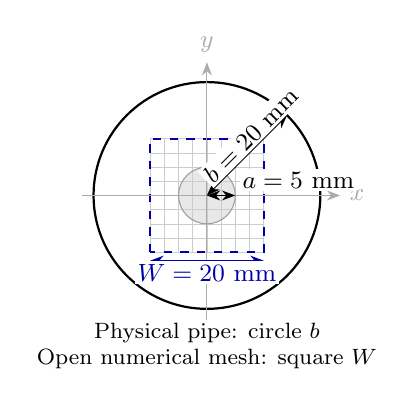
\begin{tikzpicture}[scale=.72,>=Stealth,font=\small]
 \fill[gray!18] (0,0) circle[radius=.5];
 \draw[gray!40,step=.25,very thin] (-1,-1) grid (1,1);
 \draw[blue!65!black,dashed,thick] (-1,-1) rectangle (1,1);
 \draw[black,thick] (0,0) circle[radius=2];
 \draw[gray!75] (0,0) circle[radius=.5];
 \draw[->,gray!65] (-2.2,0)--(2.35,0) node[right] {$x$};
 \draw[->,gray!65] (0,-2.2)--(0,2.35) node[above] {$y$};
 \draw[<->,black] (0,0)--(1.4142,1.4142)
   node[pos=.65,above,sloped,fill=white,inner sep=1pt] {$b=20$ mm};
 \draw[<->,black] (0,0)--(.5,0);
 \node[anchor=west,fill=white,inner sep=1pt] at (.57,.27) {$a=5$ mm};
 \draw[<->,blue!65!black] (-1,-1.15)--(1,-1.15)
   node[midway,below,fill=white,inner sep=1pt] {$W=20$ mm};
 \node[font=\footnotesize,align=center] at (0,-2.65)
   {Physical pipe: circle $b$\\Open numerical mesh: square $W$};
\end{tikzpicture}

\end{minipage}
\caption{The circle is the physical longitudinal-model pipe; the square is
the open transverse numerical grid. Distribution, beam and tracking commands
are supplied by the archived complete input. A transverse conducting wall
is not solved. For this centred round source, the local transverse image
field vanishes.}
\label{fig:pipe-model-geometry}
\end{figure}
\reportfigure{triangle-pipe-fixed-controls}{Left: radial dependence at
$s=+2.5$ m for the same selected results. Right: physical on-axis errors
under matched mesh changes. OPALX uses one source over $64^3,128^3,256^3$;
the historical PyORBIT transverse scan holds $N_z=128$ and its 16-ring source
fixed. The primary PyORBIT curve on the left uses 32 rings. Zero remains
visible; no monotonic or joint asymptotic convergence is claimed.}
{fig:triangle-pipe-fixed-controls}

All numerical changes quoted here use the 144 accepted targets. The last
matched OPALX mesh change is 0.1373\% of $E_*$. Doubling numerical width
and transverse cell count at fixed $b$ changes the field by less than
$5.5\times10^{-12}\%$; changing physical $b$ from 20 to 10 mm instead
reproduces its distinct analytic field. The initial PyORBIT ring-quadrature
bias and longitudinal sampling controls remain archived; repeated primary
results reproduce their earlier values.

Legacy \code{CIRCULAR} retains the moment coefficient
$0.67+2\ln(b/a)$~\cite{oeftiger}, with its historical width fallback when
\code{PIPERADIUS} is absent. Its unchanged lack of radial dependence explains
the earlier pointwise discrepancy. A matched legacy rerun with the new
executable agrees with its archived result within $7.4\times10^{-13}\%$ of
$E_*$. The pipe model is selected explicitly and retains the legacy CIRCULAR
closure. The later OPEN replacement is tested separately in \cref{sec:free-open}.

\clearpage
\subsection{Independent unit tests and an OPALX regression run}
\label{sec:pipe-gates}
The new physics unit tests compute the reference by integrating Gauss' law
to the grounded wall and differentiating the potential longitudinally.
They cover inside-beam, vacuum-annulus and wall fields, a non-unit Lorentz
factor, physical-radius versus mesh-width changes and rejection of particles
outside the physical pipe. Configuration tests check the explicit radius
contract and reject unsupported or inconsistent settings.

\begin{center}\small
\begin{tabular}{>{\raggedright\arraybackslash}p{0.29\linewidth}>{\raggedright\arraybackslash}p{0.63\linewidth}}
\toprule Check & Result and scope\\\midrule
C++ unit tests & 100 pass; one MPI-only test is skipped in the single-rank run.
The addition contains three independent physics tests and seven configuration
tests.\\
Reference quadrature & Independent integration/differentiation check:
maximum relative discrepancy $1.06\times10^{-11}$, below the justified
$2\times10^{-8}$ unit tolerance.\\
Native study & Six new OPALX source/probe pairs and three repeated PyORBIT
configurations. Fields, charge, positions, input and binary hashes are checked.\\
Actual OPALX regression & \code{FFT2D5-TriangularPipe} executes OPALX and checks
its H5 fields at eight nonzero targets plus two wall targets against an
independent Gauss-integral reference. Maximum physical error is 0.00352\%;
wall field is exactly zero.\\
Negative control & The same native case with the legacy model is rejected
by the physical validator; a probe-only solve confirms negligible longitudinal
probe contribution.\\
Smoke integration & STAT reference checks and the field-physics validator pass
through the local smoke runner. No remote CI execution is claimed.\\
Historical OPEN compatibility & At the pipe-update executable, ZeroSC and 1 pC regressions pass all
128 samples and six STAT reference checks with the new binary. The largest
RMS difference from their stored baseline is $4.05\times10^{-10}$ relative.\\
\bottomrule
\end{tabular}
\end{center}
The native field tolerance remains 1\%; wall targets use an absolute
$10^{-4}$ V/m tolerance because their analytic field is zero.
OPALX uses a $10^{-20}$ s readout and matched probe subtraction in the full
study. PyORBIT uses zero-charge probes and fixed-position kicks.
The repeated PyORBIT one-/two-rank fields agree within
$2.6\times10^{-12}\%$ of $E_*$; FFT2D5 remains single-rank.

The earlier benchmark is identified by binary
\begin{quote}\small
\path{e85bc09135bef40c6e0b9a278f45d9aab05ad595f2635e7c2088526bb1de70bf};
\end{quote}
the explicit pointwise model and its native tests use
\begin{quote}\small
\path{9d3771d58f0de7bf913909955e4ef81aef69a33341202edefa9553bb78ead8b5}.
\end{quote}
The before/after fine comparison uses the same physical source, targets and
$256^3$ mesh. Previous tracking and curved-tube results retain their original
binaries and interpretations.

PyORBIT slices obtain longitudinal kicks by differentiating the same grounded
slice potential used for their transverse kicks. OPALX instead combines the
analytic uniform-round $g(r)$ with its sampled $\lambda'$ and open transverse
Poisson solves. Their continuum fields coincide for this prescribed source;
this comparison does not establish a general common-potential PIC map or
symplectic tracking.

\textbf{Limit.} This validates a fixed-radius, coaxial uniform round beam's
local longitudinal pipe model on its linear density branches. Transverse
slices remain open. The model does not add nonlocal end fields, a curvature
operator or a general conducting-pipe solution. Those historical OPEN reruns test backward
compatibility only; full-drift and curved-source accuracy of the new
\code{CIRCULAR_UNIFORM} model are not established.

\clearpage
\section{Nonlocal free-space fields of the 5 m curved beam}
\label{sec:free-open}
This update addresses the historical OPEN failure in \cref{sec:frozen}.
Under the existing \code{PIPEMODE="OPEN"} interface, a new nonlocal
three-dimensional Coulomb operator replaces the independent transverse-slice
calculation and its local longitudinal closure. It includes finite-source
longitudinal coupling and circular geometry. IPPL still stores uniform
Cartesian arrays; OPALX interprets their coordinates and supplies the custom
field operator, as detailed in \cref{sec:mapped-grid}. The conducting-pipe control in
\cref{sec:triangle-pipe} tests a separate boundary model.

\subsection{Matched uniform and triangular sources}
Keep $L=5$ m, $R=2$ m, $(a,c)=(5,0.5)$ mm, $Q=10$ pC and
$\beta=0.001$. Inside the fixed elliptical section, the physical densities are
\begin{equation}
 \rho_{\rm U}=\frac{Q}{\pi acL},\qquad
 \rho_{\rm T}(s)=\frac{2Q}{\pi acL}
 \left(1-\frac{2|s|}{L}\right),\quad |s|\le L/2.
 \label{eq:free-profiles}
\end{equation}
Both vanish outside the finite tube; the uniform end is sharp. The physical
charge measure is $\dd q=\rho(s)(1+u/R)\dd u\,\dd y\,\dd s$.
No physical tail smoothing or coefficient fit enters either comparison.

SACR retains the exact Coulomb geometry. For the triangular source, integration
by parts extends \cref{eq:sacr-surface} to
\begin{equation}
 \bm E(\bm x)=\frac{1}{4\pi\eps}
 \left[\oint_{\partial V}\frac{\rho'\bm n'}{|\bm x-\bm x'|}\dd S'
 -\int_V\frac{\nabla'\rho'}{|\bm x-\bm x'|}\dd V'\right].
 \label{eq:free-weighted-sacr}
\end{equation}
The end-cap term vanishes for the triangle. The longitudinal gradient term
is integrated analytically along each filament, then by target-centred
cross-section quadrature. Side, radial and longitudinal rules are refined
independently. All 51 targets, including the cusp and added 1 mm and 0.1 mm
end-distance diagnostics, retain their stated acceptance roles.
The last nonzero-field quadrature change is below $8\times10^{-12}$ relative;
selected independent direct volume checks agree within $6\times10^{-9}$.

\subsection{One potential on a uniform reference-path coordinate grid}
Let $\kappa=1/R$, $x=u-u'$, $v=y-y'$, $\tau=s-s'$ and
\begin{equation}
 \xi(\tau)=\frac{2\sin(\kappa\tau/2)}{\kappa},\qquad
 D^2=x^2+v^2+\xi^2,\qquad
 d^2=D^2+\xi^2[\kappa(u+u')+\kappa^2uu'].
 \label{eq:free-distance}
\end{equation}
The longitudinal chord retains the full bend angle. Expanding only the small
transverse ratio $\kappa u$ gives three translation-invariant kernels,
\begin{align}
 G&=D^{-1},& H&=\xi^2D^{-3},& F&=xH,\nonumber\\
 \Phi^{(1)}&=\frac{1}{4\pi\eps}
 \left[G*\rho_{\rm FS}-\kappa u(H*\rho_{\rm FS})
       +\frac{\kappa}{2}(F*\rho_{\rm FS})\right],
 &\rho_{\rm FS}&=\frac{\dd q}{\dd u\,\dd y\,\dd s}.
 \label{eq:free-convolution}
\end{align}
Here $*$ denotes a three-dimensional convolution on the uniform $(u,y,s)$
coordinate array. The curved physical geometry enters through the custom
kernels and metric; no native curved IPPL mesh is constructed. The array
does not fill the curved beam's global Cartesian bounding box.
The same deposited density supplies every term; its Jacobian is not applied
twice. Terms quadratic in the transverse metric are omitted. All three fields
follow this common potential, $\Phi=\Phi^{(1)}$:
\begin{equation}
 E_u=-\partial_u\Phi,\qquad E_y=-\partial_y\Phi,\qquad
 E_s=-\frac{\partial_s\Phi}{1+\kappa u}.
 \label{eq:free-gradient}
\end{equation}
The flat singular source-cell integrals of $G,H,F$ are analytic. A smooth
curved-minus-flat correction is integrated numerically; fourth-order centered
differences use a two-cell potential halo. No fixed $g$ remains in OPEN.
Direct exact-versus-expanded Coulomb integration changes the weak centre
radial field by less than $3\times10^{-7}$ relative for both profiles. This
checks curvature truncation separately from mesh accuracy.
OPEN uses a smooth straight/circular coordinate map fitted to the laboratory
path and transformed with the particles. This removes polyline sagitta and
segment-frame jumps; unsupported path shapes are rejected.

\clearpage
\subsection{Native field comparison and convergence}
One native $10^{-17}$ s step with zero external field supplies each frozen
snapshot. A matched probe-only companion removes diagnostic charge; SACR is
scaled to the actual bulk charge. This is a field-operator test, not a tracking
test. The original 43 targets retain the historical comparison set, with
end distances of at least 5 mm. Here the
fixed component scales are $E_{i,*}=\max_{43}|E_i^{\rm SACR}|$ for each profile;
8 added cusp/end targets are reported separately and do not change these scales.

The table gives maximum pointwise relative errors over nonzero reference
components at the original targets. Symmetry zeros remain in the signed
fixed-scale residuals; the weak centre radial force has its own relative check.
\tabfile{free-open-errors}

\reportfigure{free-open-uniform}{Uniform physical-density tube. Black dashed:
SACR exact Coulomb identity. Lower panels show signed differences from SACR;
the gray band marks $\pm1\%$ of each fixed original-target component scale.
All zero fields remain visible.}{fig:free-open-uniform}
\reportfigure{free-open-triangle}{Same comparison for triangular physical
density, with the identical production operator and no fitted parameter.}{fig:free-open-triangle}
\subsection{Independent source, transverse-mesh and path controls}
The source refinement keeps the field mesh fixed; the transverse field-mesh
refinement then holds that refined source fixed. The path control changes
only reference sampling. The table gives maximum changes divided by each
nonzero local SACR reference field over the original 43 targets.
\tabfile{free-open-controls}
These numerical changes are separate from the absolute physical errors above.
All seven fine and control cases have maximum nonzero-target physical field
error below 0.565\% over the original 43 points.


\clearpage
\subsection{Weak curvature response, diagnostics and limits}
\reportfigure{free-open-mesh}{Matched-source longitudinal mesh refinement, with source and reference
path held fixed within each profile. Left: maximum nonzero-target physical
errors. Right: the weak signed centre radial field; dashed lines are the SACR
values, 0.055092 and 0.091839 V/m. Gray dotted: the earlier uniform slice result from its separate study,
not a matched mesh datum. Errors use their own reference components, not the
larger transverse scale.}{fig:free-open-mesh}
The additional targets include 1 mm and 0.1 mm end distances and the triangular
cusp neighbourhood. They do not alter the original acceptance scales.
\tabfile{free-open-extra}

The implementation accepts straight references or horizontal constant-radius
arcs shorter than a full turn, $\max|\kappa u|\le0.01$ across the numerical
mesh and halo, and one MPI rank. General varying-curvature paths are rejected.
Curved OPEN uses an electrostatic approximation with an explicit
$\beta\le0.1$ guard; the present validation uses $\beta=0.001$.
The operator retains the full bend angle but does not include radiation or
retarded curved-beam electrodynamics. Straight references retain their Lorentz
stretch and field transformation. No percent-level tracking claim follows.

\subsection{Repeated straight conducting-pipe control}
The same final OPALX executable reruns the independent straight benchmark in
\cref{sec:triangle-pipe}; this does not replace the free-space SACR comparison.
The fixed $1\le|s|\le4$ m window contains 62 axis and 82 beam-radial targets.
Maximum pointwise relative errors are
\tabfile{free-open-pipe-control}
The OPALX source has 8,388,608 particles. Repeated PyORBIT one-/two-rank
fields agree within $7\times10^{-9}\%$ of the local analytic field. The
maximum OPALX--PyORBIT difference is 0.447\% (slices) or 0.167\%
(Baartman). A separate native annulus/wall control has 0.00352\% maximum
nonzero-field error and exactly zero wall field. This confirms the retained
straight local pipe model; it supplies no curved free-space validation.


\clearpage
\section{Uniform IPPL grid and curved-source field operator}
\label{sec:mapped-grid}

\subsection{What the grid represents}
IPPL still stores a uniform Cartesian grid. No curved-mesh class, curved-cell
connectivity or general curvilinear Poisson solver has been added to IPPL.
The new OPALX OPEN backend interprets the three array coordinates as radial
offset $u$, vertical offset $y$ and reference-path arc length $s$. OPALX supplies
the coordinate map, the curvature-dependent Coulomb operator and the field
transformations. IPPL supplies uniform field storage and FFT operations.

\begin{figure}[H]
 \centering
 % Mapped-grid schematic, not an IPPL curved-mesh implementation.
% Physical centreline: X=((R+u)cos(s/R)-R,y,(R+u)sin(s/R)); R=2 m.
% The origin of s is shifted to the charged-beam midpoint for this figure.
% Visible physical tube thickness and grid spacing are deliberately schematic.
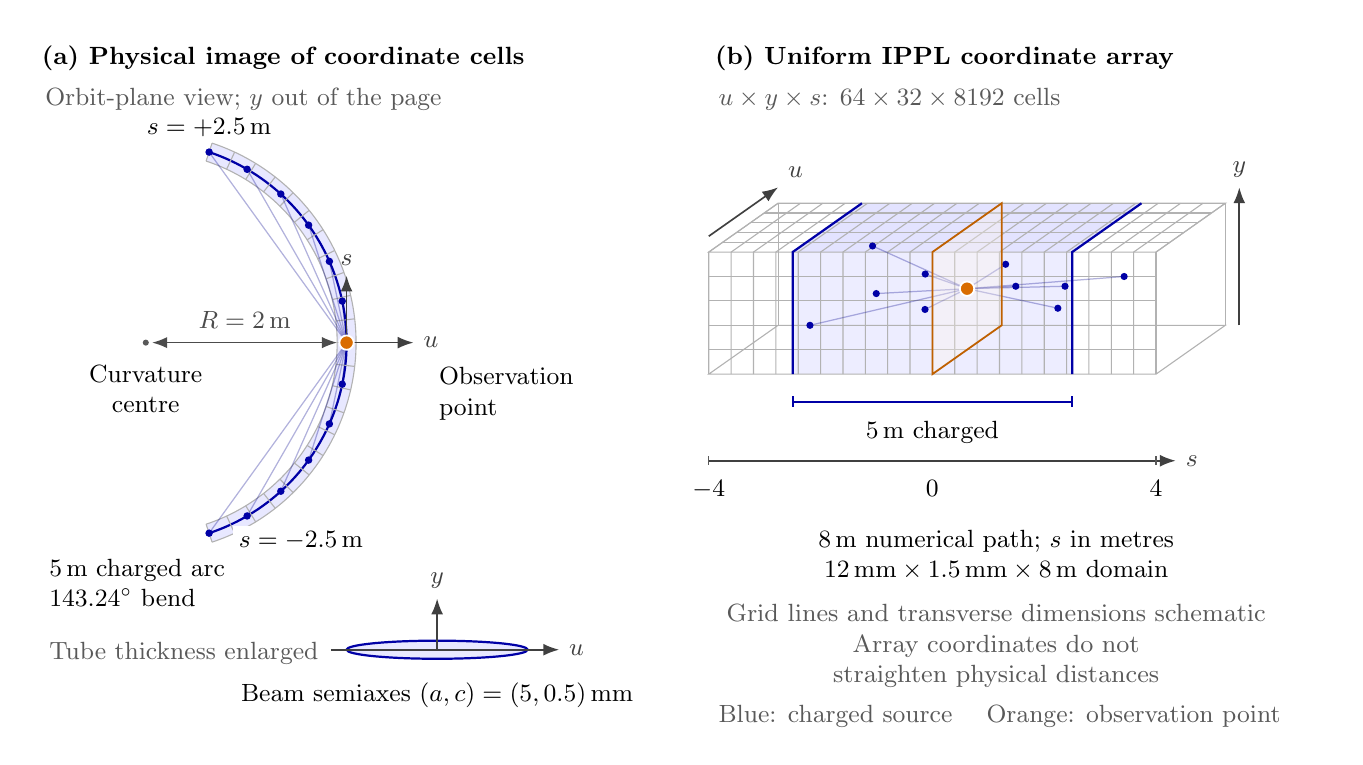
\begin{tikzpicture}[
  x=1cm,y=1cm,font=\small,>=Latex,
  mggrid/.style={line width=.4pt,black!30},
  mgsource/.style={blue!65!black,line width=.8pt},
  mgcoupling/.style={blue!55!black,opacity=.3,line width=.45pt},
  mgaxis/.style={->,black!75,line width=.6pt},
  mgdim/.style={<->,black!70,line width=.55pt},
  mgtarget/.style={fill=orange!85!black,draw=white,line width=.65pt},
  mglabel/.style={fill=white,inner sep=2pt}
]
 \path[use as bounding box] (0,0) rectangle (16.6,9.0);
 \node[anchor=north west,font=\bfseries\small,align=left,text width=7.4cm]
   at (.1,8.9) {(a) Physical image of coordinate cells};
 \node[anchor=north west,font=\bfseries\small,align=left,text width=7.7cm]
   at (8.65,8.9) {(b) Uniform IPPL coordinate array};
 \node[anchor=north west,black!65] at (.1,8.35)
   {Orbit-plane view; $y$ out of the page};
 \node[anchor=north west,black!65] at (8.65,8.35)
   {$u\times y\times s$: $64\times32\times8192$ cells};

 % Physical circular arc: theta=s/R, -1.25 <= theta <= 1.25 rad.
 \coordinate (mgO) at (1.5,5.0);
 \coordinate (mgT) at ($(mgO)+(0:2.55)$);
 \fill[blue!9] ($(mgO)+(-71.619724:2.43)$)
   arc[start angle=-71.619724,end angle=71.619724,radius=2.43]
   -- ($(mgO)+(71.619724:2.67)$)
   arc[start angle=71.619724,end angle=-71.619724,radius=2.67] -- cycle;
 \foreach \rad in {2.43,2.67} {
   \draw[mggrid] ($(mgO)+(-71.619724:\rad)$)
     arc[start angle=-71.619724,end angle=71.619724,radius=\rad];
 }
 \draw[mgsource] ($(mgO)+(-71.619724:2.55)$)
   arc[start angle=-71.619724,end angle=71.619724,radius=2.55];
 \foreach \theta in {-71.619724,-65,-58.5,-52,-45.5,-39,-32.5,-26,-19.5,-13,-6.5,0,6.5,13,19.5,26,32.5,39,45.5,52,58.5,65,71.619724} {
   \draw[mggrid] ($(mgO)+(\theta:2.43)$) -- ($(mgO)+(\theta:2.67)$);
 }
 \foreach \theta in {-71.619724,-59.6831,-47.7465,-35.8099,-23.8732,-11.9366,11.9366,23.8732,35.8099,47.7465,59.6831,71.619724} {
   \draw[mgcoupling] ($(mgO)+(\theta:2.55)$) -- (mgT);
   \fill[blue!65!black] ($(mgO)+(\theta:2.55)$) circle[radius=1.35pt];
 }
 \fill[black!65] (mgO) circle[radius=1.1pt];
 \draw[mgdim] ($(mgO)+(.08,0)$) -- ($(mgT)+(-.12,0)$)
   node[midway,above=3pt,mglabel] {$R=2\,\mathrm m$};
 \node[anchor=north,align=center] at ($(mgO)+(0,-.16)$)
   {Curvature\\centre};
 \draw[mgaxis] (mgT) -- ($(mgT)+(.85,0)$) node[right] {$u$};
 \draw[mgaxis] (mgT) -- ($(mgT)+(0,.85)$) node[above] {$s$};
 \fill[mgtarget] (mgT) circle[radius=2.6pt];
 \node[anchor=west,align=left] at ($(mgT)+(1.05,-.65)$)
   {Observation\\point};
 \node[anchor=south,mglabel] at ($(mgO)+(71.619724:2.55)+(0,.12)$)
   {$s=+2.5\,\mathrm m$};
 \node[anchor=west,mglabel] at ($(mgO)+(-71.619724:2.55)+(.3,-.1)$)
   {$s=-2.5\,\mathrm m$};
 \node[anchor=west,align=left] at (.15,1.95)
   {$5\,\mathrm m$ charged arc\\$143.24^\circ$ bend};
 \node[anchor=west,black!65] at (.15,1.05)
   {Tube thickness enlarged};

 % True transverse aspect ratio a/c=10, drawn at a separate magnification.
 \coordinate (mgS) at (5.2,1.1);
 \draw[mgsource,fill=blue!9] (mgS) ellipse[x radius=1.15,y radius=.115];
 \draw[mgaxis] ($(mgS)+(-1.35,0)$) -- ($(mgS)+(1.55,0)$) node[right] {$u$};
 \draw[mgaxis] (mgS) -- ($(mgS)+(0,.65)$) node[above] {$y$};
 \node[anchor=north,align=center] at ($(mgS)+(0,-.3)$)
   {Beam semiaxes $(a,c)=(5,0.5)\,\mathrm{mm}$};

 % A rectangular array in logical coordinates. s is long; u is the slanted
 % depth direction; y is vertical. Physical aspect ratios are not drawn to scale.
 \begin{scope}[shift={(8.65,4.6)},x={(.71cm,0cm)},y={(.88cm,.62cm)},z={(0cm,1.55cm)}]
   \fill[blue!11] (1.5,0,1) -- (6.5,0,1) -- (6.5,1,1) -- (1.5,1,1) -- cycle;
   \fill[blue!7] (1.5,0,0) -- (6.5,0,0) -- (6.5,0,1) -- (1.5,0,1) -- cycle;
   \draw[mggrid] (0,0,0) -- (8,0,0) -- (8,1,0) -- (0,1,0) -- cycle;
   \draw[mggrid] (0,0,1) -- (8,0,1) -- (8,1,1) -- (0,1,1) -- cycle;
   \foreach \ss in {0,8} {
     \foreach \uu in {0,1} {\draw[mggrid] (\ss,\uu,0) -- (\ss,\uu,1);}
   }
   \foreach \ss in {0,.4,...,8} {
     \draw[mggrid] (\ss,0,0) -- (\ss,0,1) -- (\ss,1,1);
   }
   \foreach \qq in {.2,.4,.6,.8} {
     \draw[mggrid] (0,0,\qq) -- (8,0,\qq);
     \draw[mggrid] (0,\qq,1) -- (8,\qq,1);
   }
   \foreach \ss in {1.5,6.5} {
     \draw[mgsource] (\ss,0,0) -- (\ss,0,1) -- (\ss,1,1);
   }
   \foreach \ss/\uu/\yy in {1.5/.25/.3,2/.75/.75,2.5/.4/.5,3/.7/.25,3.5/.3/.7,4.5/.8/.4,5/.25/.8,5.5/.6/.3,6/.3/.6,6.5/.75/.5} {
     \draw[mgcoupling] (\ss,\uu,\yy) -- (4,.5,.5);
     \fill[blue!65!black] (\ss,\uu,\yy) circle[radius=1.3pt];
   }
   \draw[orange!75!black,line width=.65pt,fill=orange!7,fill opacity=.35]
     (4,0,0) -- (4,0,1) -- (4,1,1) -- (4,1,0) -- cycle;
   \fill[mgtarget] (4,.5,.5) circle[radius=2.6pt];
   \draw[mgaxis] (0,0,1.13) -- (0,1,1.13) node[above right] {$u$};
   \draw[mgaxis] (8.25,1,0) -- (8.25,1,1.13) node[above] {$y$};
   \coordinate (mgAL) at (0,0,0);
   \coordinate (mgAR) at (8,0,0);
   \coordinate (mgCL) at (1.5,0,0);
   \coordinate (mgCR) at (6.5,0,0);
 \end{scope}
 \draw[mgsource] ($(mgCL)+(0,-.35)$) -- ($(mgCR)+(0,-.35)$);
 \foreach \pp in {mgCL,mgCR} {\draw[mgsource] ($(\pp)+(0,-.28)$) -- ($(\pp)+(0,-.42)$);}
 \node[anchor=north] at ($(mgCL)!.5!(mgCR)+(0,-.48)$) {$5\,\mathrm m$ charged};
 \draw[mgaxis] ($(mgAL)+(0,-1.1)$) -- ($(mgAR)+(.25,-1.1)$) node[right] {$s$};
 \foreach \pp/\val in {mgAL/-4,mgAR/4} {
   \draw[black!65,line width=.5pt] ($(\pp)+(0,-1.04)$) -- ($(\pp)+(0,-1.16)$);
   \node[anchor=north] at ($(\pp)+(0,-1.23)$) {$\val$};
 }
 \node[anchor=north] at ($(mgAL)!.5!(mgAR)+(0,-1.23)$) {$0$};
 \node[align=center] at (12.3,2.3)
   {$8\,\mathrm m$ numerical path; $s$ in metres\\
    $12\,\mathrm{mm}\times1.5\,\mathrm{mm}\times8\,\mathrm m$ domain};
 \node[align=center,black!65,text width=7.5cm] at (12.3,1.15)
   {Grid lines and transverse dimensions schematic\\
    Array coordinates do not straighten physical distances};
 \node[anchor=west,black!65] at (8.65,.25)
   {Blue: charged source \quad Orange: observation point};
\end{tikzpicture}

 \caption{Two representations of the same source. Left: the physical image of
 reference-path coordinate cells on a circular arc, with transverse thickness
 enlarged. Right: the ordinary rectangular IPPL array indexed by $(u,y,s)$.
 The rectangular drawing does not straighten the source in the Coulomb
 calculation. Lines joining source sections to an observation point illustrate
 nonlocal coupling, not computed field vectors or magnitudes. Only a schematic
 subset of grid lines is drawn; the empty interior of the bend is not meshed.}
 \label{fig:mg-geometry}
\end{figure}

\begin{center}\small
\begin{tabular}{ll}\toprule
Quantity & Frozen-field benchmark\\\midrule
Charged length; bending radius & $L=5$ m; $R=2$ m\\
Total source angle; radial thinness & $L/R=2.5$ rad $=143.24^\circ$; $a/R=0.0025$\\
Radial / vertical source semiaxes & $a=5$ mm; $c=0.5$ mm\\
Uniform coordinate domain & $12$ mm $\times1.5$ mm $\times8$ m\\
Primary field grid & $64\times32\times8192$ cells\\\bottomrule
\end{tabular}
\end{center}

This is a nonlocal three-dimensional field calculation specialized to a thin
circular tube, selected through the existing \code{FFT2D5} interface. It
replaces the OPEN slice calculation; it is more than a correction to a local
longitudinal coefficient. The other pipe modes retain their separate slice
calculations and longitudinal closures.

\clearpage
\subsection{Coordinate map and charge deposition}
For an explanatory circle centred at $(-R,0,0)$, choose $s=0$ at the middle
of the charged arc and define
\begin{equation}
 \bm X(u,y,s)=
 \begin{pmatrix}(R+u)\cos(s/R)-R\\ y\\(R+u)\sin(s/R)\end{pmatrix},
 \qquad -L/2\le s\le L/2.
 \label{eq:mg-map}
\end{equation}
The implementation instead starts $s=0$ at the first reference-path point.
An arc-length origin shift and a rigid rotation/translation connect the two
conventions. They do not change source-target separations or the calculation.
Path and particle coordinates are placed in one common solve frame.

For $\kappa=1/R$, the local radial, vertical and tangent unit vectors are
\begin{equation}
 \bm e_u=(\cos\kappa s,0,\sin\kappa s),\quad
 \bm e_y=(0,1,0),\quad
 \bm e_s=(-\sin\kappa s,0,\cos\kappa s).
 \label{eq:mg-basis}
\end{equation}
The coordinate scale factors are $(1,1,h)$, where
\begin{equation}
 h(u)=1+\kappa u,\qquad
 \dd\ell^2=\dd u^2+\dd y^2+h^2\dd s^2,\qquad
 \dd V=h\,\dd u\,\dd y\,\dd s.
 \label{eq:mg-metric}
\end{equation}
Thus uniform intervals in $s$ are uniform reference-path arc intervals.
At a radial offset $u$, their physical tangential length is $h\,\Delta s$.
The mapped physical cells have different tangential lengths even though the
IPPL coordinate spacing is constant.

OPALX first maps each particle position to $(u,y,s)$ and then applies ordinary
cloud-in-cell deposition on that uniform coordinate grid. Its cell centres are
\begin{equation}
 (u_i,y_j,s_k)=
 (u_{\min}+(i+\tfrac12)\Delta u,\;
  y_{\min}+(j+\tfrac12)\Delta y,\;
  s_{\min}+(k+\tfrac12)\Delta s).
 \label{eq:mg-grid}
\end{equation}
The primary spacings are $\Delta u=0.1875$ mm, $\Delta y=0.046875$ mm and
$\Delta s=0.9765625$ mm. The stored source is charge per \emph{coordinate}
volume, not charge per physical volume:
\begin{equation}
 \rho_c=\frac{\dd q}{\dd u\,\dd y\,\dd s}
       =h\rho_{\rm phys},\qquad
 \int\rho_c\,\dd u\,\dd y\,\dd s=Q.
 \label{eq:mg-density}
\end{equation}
Depositing actual particle charges already represents this Jacobian. Applying
an additional factor $h$ to the deposited source would count it twice. A
uniform physical density therefore corresponds to coordinate density
proportional to $h$, rather than a constant array value.

Merely mapping coordinates and calling a Cartesian Poisson solver would omit
the geometric terms. For constant curvature, the physical Laplacian is
\begin{equation}
 \nabla^2\Phi=\frac1h\partial_u(h\partial_u\Phi)
       +\partial_y^2\Phi+\frac1{h^2}\partial_s^2\Phi.
 \label{eq:mg-laplacian}
\end{equation}
The current backend does not discretize this mapped PDE. It instead constructs
an approximate physical free-space Green function and evaluates its integral.

\clearpage
\subsection{How the curved Coulomb interaction becomes FFT convolutions}
In the low-speed curved case, the electrostatic potential is
\begin{equation}
 \Phi(u,y,s)=\frac1{4\pi\eps}
 \int\frac{\rho_c(u',y',s')}{d(u,y,s;u',y',s')}
           \,\dd u'\,\dd y'\,\dd s',
 \label{eq:mg-exact-potential}
\end{equation}
where $d=|\bm X(u,y,s)-\bm X(u',y',s')|$ is a physical Cartesian distance.
For a circular reference, introduce $x=u-u'$, $v=y-y'$ and $\tau=s-s'$.
The exact squared distance is
\begin{align}
 \xi(\tau)&=\frac{2\sin(\kappa\tau/2)}{\kappa},\qquad
 D^2=x^2+v^2+\xi^2,\nonumber\\
 d^2&=x^2+v^2+\xi^2(1+\kappa u)(1+\kappa u')
     =D^2+\xi^2[\kappa(u+u')+\kappa^2uu'].
 \label{eq:mg-distance}
\end{align}
The chord $\xi$ retains the full angular separation. At the two source ends,
$|\tau|=5$ m gives a centreline chord of $3.79594$ m, rather than the 5 m
arc length. A small transverse ratio $a/R$ therefore does not justify
replacing the strongly bent source by a straight beam.

The exact kernel depends separately on $u$ and $u'$ through their metric
factors. It is \emph{not} a single translation-invariant convolution in all
three logical coordinates. The implementation expands in small transverse
curvature, while retaining the full chord:
\begin{equation}
 \frac1d\simeq G-\frac\kappa2(u+u')H,
 \qquad G=D^{-1},\quad H=\xi^2D^{-3},\quad F=xH.
 \label{eq:mg-expansion}
\end{equation}
Using $u'=u-x$ rewrites the first-order kernel as
$G-\kappa uH+\kappa F/2$. Each of $G,H,F$ now depends only on
$(u-u',y-y',s-s')$. With $*$ denoting three-dimensional convolution,
\begin{equation}
 \boxed{\displaystyle
 \Phi^{(1)}=\frac1{4\pi\eps}
 \left[G*\rho_c-\kappa u(H*\rho_c)+\frac\kappa2(F*\rho_c)\right].}
 \label{eq:mg-three-convolutions}
\end{equation}
The remaining factor $u$ is applied at the observation cell after convolution.
This decomposition, rather than a curved IPPL mesh, enables the FFT method.
No fitted geometry factor or prescribed uniform/triangular profile enters
the production kernel.

At $\kappa\to0$, $\xi\to\tau$ and the correction terms vanish, recovering
the ordinary three-dimensional Coulomb kernel. At finite curvature the
operator is approximate: quadratic transverse-curvature terms are omitted.
Small potential truncation error does not guarantee the same relative error
in a weak field component formed by cancellation; componentwise reference
checks remain necessary. General varying-curvature paths do not have this
simple three-convolution form and are not implemented.

\clearpage
\subsection{What IPPL computes and how fields return to particles}
\begin{figure}[H]
 \centering
 % Ownership of geometry/physics and of uniform-grid/FFT infrastructure.
% No generic curvilinear IPPL Poisson operator is used in this pipeline.
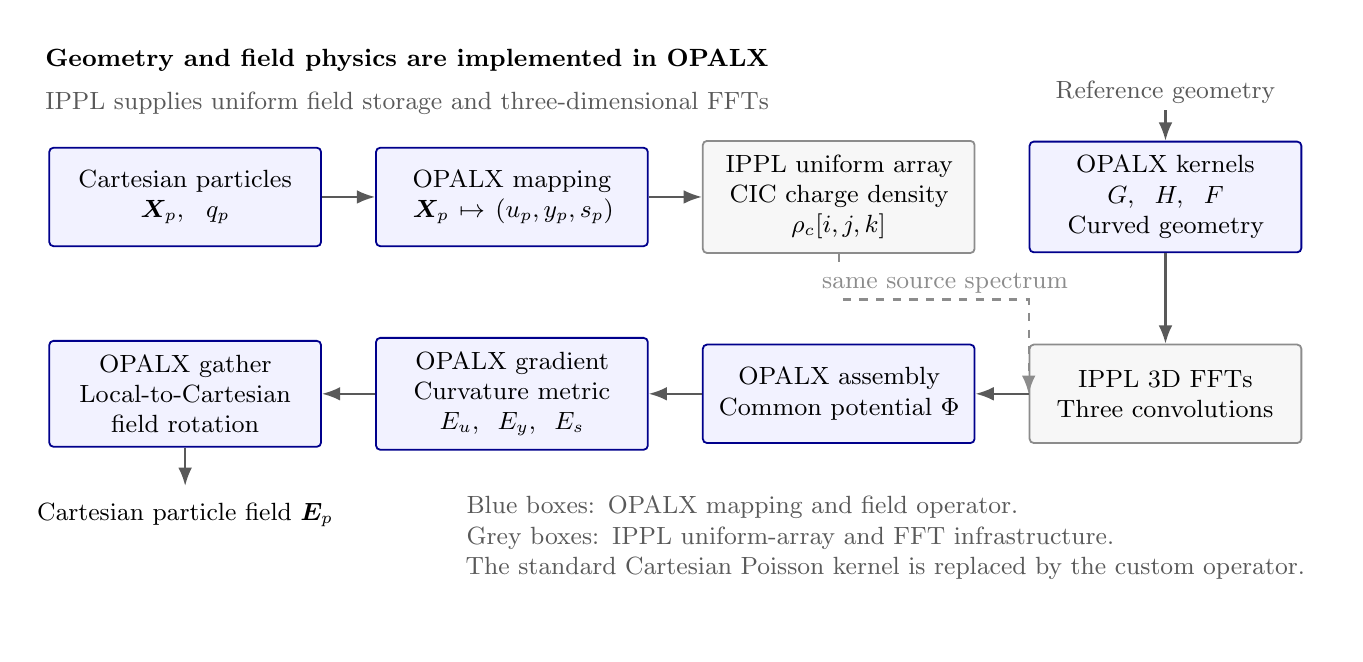
\begin{tikzpicture}[
 x=1cm,y=1cm,font=\small,>=Latex,
 mgop/.style={draw=blue!55!black,fill=blue!5,line width=.65pt,
   rounded corners=1.5pt,align=center,text width=3.1cm,minimum height=1.25cm,inner sep=5pt},
 mgippl/.style={draw=black!45,fill=black!3,line width=.65pt,
   rounded corners=1.5pt,align=center,text width=3.1cm,minimum height=1.25cm,inner sep=5pt},
 mgflow/.style={->,line width=.8pt,black!65},
 mgflowlabel/.style={fill=white,inner sep=2pt,align=center}
]
 \path[use as bounding box] (0,0) rectangle (16.6,7.7);
 \node[anchor=north west,font=\bfseries\small] at (.1,7.55)
   {Geometry and field physics are implemented in OPALX};
 \node[anchor=north west,black!65] at (.1,7.0)
   {IPPL supplies uniform field storage and three-dimensional FFTs};

 \node[mgop] (mga) at (2.0,5.55)
   {Cartesian particles\\$\bm X_p,\;q_p$};
 \node[mgop] (mgb) at (6.15,5.55)
   {OPALX mapping\\$\bm X_p\mapsto(u_p,y_p,s_p)$};
 \node[mgippl] (mgc) at (10.3,5.55)
   {IPPL uniform array\\CIC charge density\\$\rho_c[i,j,k]$};
 \node[mgop] (mgd) at (14.45,5.55)
   {OPALX kernels\\$G,\;H,\;F$\\Curved geometry};
 \draw[mgflow] (mga) -- (mgb);
 \draw[mgflow] (mgb) -- (mgc);
 \draw[mgflow] (14.45,6.65) -- (mgd.north)
   node[pos=0,above,mgflowlabel] {Reference geometry};

 \node[mgippl] (mge) at (14.45,3.05)
   {IPPL 3D FFTs\\Three convolutions};
 \node[mgop] (mgf) at (10.3,3.05)
   {OPALX assembly\\Common potential $\Phi$};
 \node[mgop] (mgg) at (6.15,3.05)
   {OPALX gradient\\Curvature metric\\$E_u,\;E_y,\;E_s$};
 \node[mgop] (mgh) at (2.0,3.05)
   {OPALX gather\\Local-to-Cartesian\\field rotation};
 \draw[mgflow] (mgd) -- (mge);
 \draw[mgflow] (mge) -- (mgf);
 \draw[mgflow] (mgf) -- (mgg);
 \draw[mgflow] (mgg) -- (mgh);

 \node[anchor=north,align=center] at (2.0,1.78)
   {Cartesian particle field $\bm E_p$};
 \draw[mgflow] (mgh.south) -- (2.0,1.88);
 \draw[mgflow,dashed,black!45] (mgc.south) -- ++(0,-.58) -| (mge.west)
   node[pos=.28,above,mgflowlabel] {same source spectrum};
 \node[anchor=west,text width=10.7cm,align=left,black!65] at (5.45,1.22)
   {Blue boxes: OPALX mapping and field operator.\\
    Grey boxes: IPPL uniform-array and FFT infrastructure.\\
    The standard Cartesian Poisson kernel is replaced by the custom operator.};
\end{tikzpicture}

 \caption{Division of responsibility in the implemented OPEN calculation.
 OPALX handles the physical geometry, source interpretation, custom kernels,
 metric gradient and field rotations. IPPL stores ordinary uniform arrays
 and performs FFTs. The existing Cartesian Poisson operator is not used for
 this curved-source convolution.}
 \label{fig:mg-pipeline}
\end{figure}

The source array is transformed once per solve. For each of $G,H,F$, the
backend constructs the cell-integrated kernel, transforms it, multiplies its
spectrum by the same source spectrum, inverse-transforms and accumulates the
appropriate term of \cref{eq:mg-three-convolutions}. FFT plans and work arrays
persist while the mesh shape and spacing remain unchanged. A straight source
needs only $G$; the curved source uses all three kernels.

The discrete FFT is periodic algebraically, so the code embeds the density
in zero-padded arrays to evaluate a free-space linear convolution. In each
direction, the padded length is an even 2/3/5-smooth integer at least $2N+4$.
The extra support accommodates the two-cell potential halo. This numerical
padding does not introduce a physical conducting boundary or a periodic beam.
The singular flat-cell kernel integrals are analytic; a smooth
curved-minus-flat correction is evaluated by quadrature.

For the curved electrostatic case, all local electric components come from
the same potential:
\begin{equation}
 E_u=-\partial_u\Phi^{(1)},\qquad
 E_y=-\partial_y\Phi^{(1)},\qquad
 E_s=-\frac1h\partial_s\Phi^{(1)}.
 \label{eq:mg-field}
\end{equation}
Physical-cell derivatives use fourth-order centred differences. OPALX
interpolates these components to each particle in logical coordinates and
then rotates them into Cartesian directions:
\begin{equation}
 \bm E_{\rm Cartesian}
 =E_u\bm e_u(s)+E_y\bm e_y+E_s\bm e_s(s).
 \label{eq:mg-rotate}
\end{equation}
The geometry used for mapping, field evaluation and rotation is consistent
within one common solve frame. Interpolating without the metric factor, or
returning local components as fixed Cartesian components, would change the
physical result.

\clearpage
\subsection{Computational cost and the change from a slice model}
The conventional slice calculation solves transverse Poisson problems
independently and supplies a separate local longitudinal approximation.
The revised OPEN backend couples the entire deposited three-dimensional
source. It retains the FFT2D5 interface and reference-path organization, but
has genuine three-dimensional FFT cost.

\begin{center}\small
\begin{tabular}{p{0.21\linewidth}p{0.33\linewidth}p{0.36\linewidth}}\toprule
Property & Retained slice/pipe calculation & Revised free-space OPEN\\\midrule
Transverse coupling & Within each transverse slice & Across the finite source\\
Longitudinal field & Separate local closure & Gradient of a common nonlocal potential\\
Numerical transforms & Repeated transverse 2D FFTs & Three-coordinate FFT convolutions\\
Geometry treatment & Local reference-path slices & Smooth circular map and first-order curved-source kernel\\
PyORBIT control & Straight conducting-pipe longitudinal model & Not a curved free-space cross-code comparison\\\bottomrule
\end{tabular}
\end{center}

For $N=N_uN_yN_s$, a three-dimensional transform scales as $O(N\log N)$,
with additional work for the three kernel convolutions. Padding is required
in all three directions. Persistent convolution storage includes one padded
real field, two half-complex fields and an unpadded potential with a halo;
the deposited fields, particle arrays and FFT workspaces add further memory.
Measured peak native-run memory was approximately 13.8 GB for
$64\times32\times8192$ and 27.1 GB for $96\times48\times8192$.
These are whole-run measurements, not the byte count of one grid or a
universal memory forecast.

The reference-path coordinates still save the large empty space inside the
bend. A Cartesian box spanning metre-scale orbit dimensions would require
many cells unrelated to the millimetre-scale beam cross-section if comparable
resolution were imposed. The coordinate-array approach avoids that geometric
cost, but does not retain the computational cost of independent 2D slices.

Nonlocal source coupling is needed to reproduce the finite curved Coulomb
reference being tested. A 3D FFT is one way to evaluate it, not a mathematical
necessity. A reduced approach could combine local transverse solves with a
nonlocal longitudinal/curvature correction or a hierarchical interaction
method. Such an efficient replacement has not been demonstrated here.
Agreement of the present OPEN backend with SACR therefore validates a
different, more expensive operator; it does not prove that the earlier
inexpensive slice approximation meets the same curved-beam target.

\clearpage
\subsection{Validation scope, restrictions and code correspondence}
The completed comparison uses $Q=10$ pC, $\beta=0.001$, the geometry in
\cref{fig:mg-geometry} and uniform or triangular physical longitudinal density.
It tests native particle deposition, solution and gathering against the
independent exact-geometry SACR reference. The primary-grid maximum pointwise
relative errors over the original 43 sampled positions per profile are
\begin{center}\small
\begin{tabular}{lrrr}\toprule
Profile & Radial $E_u$ & Vertical $E_y$ & Tangential $E_s$\\\midrule
Uniform & 0.07084\% & 0.07789\% & 0.55443\%\\
Triangular & 0.06613\% & 0.08660\% & 0.08299\%\\\bottomrule
\end{tabular}
\end{center}
Those positions are at least 5 mm inside the source ends. Across the seven
qualified fine/control cases, the worst nonzero-component relative error is
0.56413\%. The extra uniform-source diagnostic 0.1 mm inside a sharp end
still has 20.66\% tangential error. There is no claim of 1\% accuracy at every
position, or of validated self-consistent tracking.

The current implementation has the following restrictions:
\begin{itemize}
 \item Straight references or horizontal constant-curvature circular arcs
 shorter than one turn, followed by a common rigid solve-frame transformation.
 General paths and closed rings are rejected; near-full-turn accuracy is untested.
 \item One MPI rank and $\max|\kappa u|\le0.01$ across the coordinate domain
 and two-cell potential halo. Every source particle needs a half-cell CIC margin.
 \item Curved fields use instantaneous electrostatics. The code rejects
 $\beta>0.1$, but that cutoff is not a componentwise 1\% error guarantee.
 The local magnetic-field prescription is not a nonlocal Biot--Savart solve;
 retardation, radiation and relativistic curved tracking are unvalidated.
 \item Straight references instead use a common mean-$\gamma$ longitudinal
 stretch and field transformation. The curved formulas above use $\gamma=1$.
\end{itemize}

\begin{center}\small
\begin{tabular}{p{0.43\linewidth}p{0.51\linewidth}}\toprule
Implementation component & Responsibility\\\midrule
\code{FFT2D5Geometry} & Fit supported references; map positions and construct the local basis\\
\code{FFT2D5FieldStorage} & Uniform IPPL coordinate arrays and retained slice workspace\\
\code{FFT2D5Algorithm} & Common solve frame, CIC deposition/gathering, coverage checks and rotations\\
\code{FFT2D5FreeSpaceKernel.h} & Cell-integrated $G,H,F$ kernels and curved chord\\
\code{FFT2D5FreeSpace} & Padded 3D FFT convolutions, potential assembly and metric gradient\\\bottomrule
\end{tabular}
\end{center}
The separate straight conducting-pipe comparison with PyORBIT tests the
retained local model: its maximum OPALX--PyORBIT slice-field difference is
0.447\%. It is not independent cross-code validation of this nonlocal curved
OPEN operator. No simulation or production-code change is introduced by this
explanation.


\clearpage
\appendix
\section{Software verification and automated tracking checks}
\label{app:verification}
\begin{center}\small
\begin{tabular}{>{\raggedright\arraybackslash}p{0.29\linewidth}>{\raggedright\arraybackslash}p{0.63\linewidth}}\toprule
Check & Result and scope\\\midrule
Independent model & Sphere, oblate and integral checks; zero-charge rotation,
centroid, invariants, positive volume and tighter integration pass.\\
Earlier C++ unit tests & 131/131 CTest entries pass with one OpenMP thread. Tests cover
kernels, forces, halos, boundaries, small grids, neutral/empty sources and frames.\\
Four-thread numerics & 66 applicable tests pass; the MPI-only guard is skipped
in this single-rank run.\\
Two-rank FFT2D5 guard & Unsupported-MPI rejection passes. Distributed FFT2D5
tracking is not tested; GPU execution is unverified.\\
3D OPEN tracking & Baseline one-/two-rank curves agree within
$3.5\times10^{-13}$ relative. Completed 10 pC OPEN sizes agree with the model
within 0.070\%.\\
10 pC controls & All five runs complete, including both zero controls;
80 particle snapshots pass independent count, charge, field-map and diagnostic checks.\\
SACR fields & 33 points in each of three geometries; the 5 m source also uses
11 bend-radius values. Static field and quadrature checks are separate from
OPALX tracking. See \cref{sec:sacr}.\\
Frozen curved tube & Native one-rank fields at 43 points, separate transverse
and longitudinal mesh scans, and source/path controls. Integrity checks pass;
the 1\% physical field target fails. See \cref{sec:frozen}.\\
Earlier tracking regressions & ZeroSC and 1 pC all-step validators pass locally.
The original study ran only ZeroSC through the full smoke hook;
updated compatibility checks are in \cref{sec:pipe-gates}.\\
Validator integration & Seven runner tests and six deliberately corrupted
tracking outputs pass their expected acceptance/rejection checks.\\
Remote CI & Cases and workflow remain local and unpublished. The external
CSCS runner retains its existing \code{.rt} checks.\\\bottomrule
\end{tabular}
\end{center}
\tabfile{modelchecks}

The OPALX tracking cases \code{FFT2D5-UniformB-ZeroSC} and
\code{FFT2D5-UniformB-1pC} check all 128 STAT samples against the independent
model, plus duration, particle count, assigned charge and source fixtures.
Corruption controls alter an intermediate RMS, particle count, charge, time,
finite values or output length. These checks supplement the three final-value
\code{.rt} checks. Tracking regressions and C++ unit tests are separate test layers.

\subsection{Incomplete runs}
\begin{center}\small
\begin{tabular}{lrrl}\toprule
Case & STAT rows & Duration covered & Intended check\\\midrule
$R=0.25$ m fine mesh & 61/128 & 47.6563\% & $256\times512\times550$\\\bottomrule
\end{tabular}
\end{center}
This run remains excluded from acceptance. The earlier interrupted 10 pC
files are preserved, but complete replacement runs now supply the results in
Section~6. Report generation launches no simulations.

\subsection{Historical slice implementation}
The earlier solver uses the rectangular-cell-averaged logarithmic Green function,
including the finite self-cell, and centered gradients with convolved potential
halos. It transforms particles and the laboratory reference path into a common
solve frame, then restores the particle frame. One FFT workspace serves all
slices; cleared empty slices are skipped, while nonempty neutral sources are solved.

\subsection{Nonlocal OPEN verification}
Six selected CTest executables pass 113 unit tests; 1 MPI-only test
is skipped in the one-rank invocation and passes separately on two ranks.
FFT2D5 therefore still rejects unsupported distributed execution. Backend
checks include a finite source-cell self integral and independent ellipsoid
fields at $\gamma=1,2$; geometry and frame checks are separate from native
physical-field convergence. No existing physical tolerance was relaxed.

Weighted checkpoint sources require preserving each particle's charge and
mass. An auxiliary fix prevents the emission stage from overwriting these
attributes when no emitter is active. Independent sorted-ID audits verify
q/m, total weighted charge, source geometry and frozen motion for both final
profiles. The pre-fix smoke run changed the profile and is explicitly invalid;
it supplies no field-accuracy evidence. The existing header charge diagnostic
can be wrong for nonuniform weights; source normalization uses the actual
sum of particle weights and never that header value.


\subsection{Evidence catalog}
Paths below are relative to \code{data/}; CSV values retain their stored precision.
\begin{center}\footnotesize
\begin{tabular}{>{\raggedright\arraybackslash}p{0.25\linewidth}>{\raggedright\arraybackslash}p{0.67\linewidth}}\toprule
Result & Evidence files\\\midrule
Baseline/refinements & \code{baseline-summary.csv}, \code{baseline-convergence.csv},
\code{baseline-acceptance.json}\\
3D OPEN controls & \code{open-summary.csv}, \code{open-refinement-summary.csv},
\code{open-convergence.json}\\
Completed 10 pC study & \code{10pc-completed/}: all-step sizes/growth,
refinement, covariance/centroid, five manifests and particle verification\\
SACR field reference & \code{sacr/}: point set, field values, quadrature and
radius summaries, code/provenance and independent differential/volume checks\\
Frozen 5 m tube & \code{frozen-r2/}: constant-section reference, all-component
fields, matched mesh/control data, native end profiles and plotting sources\\
Corrected OPEN profiles & \code{free-open/}: uniform/triangular SACR fields,
native full/probe tables, matched-source mesh scan, independent q/m audits,
compact source quadratures, code/build provenance and repeated pipe controls\\
Literature comparison & \code{literature/}: primary-source review/synthesis
metadata and hashes; linked references appear in the bibliography\\
Collective response & \code{growth-summary.csv}, \code{centroid-summary.csv},
\code{covariance-snapshots.csv}\\
Initial fields / $g$ & \code{field-summary.csv}, \code{g-evolution.csv}\\
Radius scan & \code{radius-summary.csv}, \code{radius-all-case-summary.csv},
\code{analytic-geometry.csv}\\
Model and generator & \code{model-checks.json}, \code{strong-model-checks.json},
\code{ellipsoid_model.py}, \code{prepare_opalx.py}\\
Software checks & \code{test-logs/fft2d5-final-*.log},
\code{zero-regression-validation.json}, \code{q1-regression-validation.json}\\
Incomplete runs & \code{incomplete-manifests/}\\\bottomrule
\end{tabular}
\end{center}

\clearpage
\section{Reproduction and provenance}
The earlier frame/slice fix is saved locally in commit \code{fd6ba8dc5} on
\code{658-fft2d5-keep-particles-and-reference-path-in-a-consistent-frame}.
Later validation/report edits remain uncommitted. Baseline and radius results
use the archived tracking binary
\begin{quote}\small
\path{ba08fdd0b0bb1e90a64ba0fd3763a8b6d044b128c0af9b9dfd215ad0ffac8fd4}.
\end{quote}
The completed 10 pC study pins a second build of the same twelve solver/test
sources, with SHA-256
\begin{quote}\small
\path{e85bc09135bef40c6e0b9a278f45d9aab05ad595f2635e7c2088526bb1de70bf}.
\end{quote}
Its coarse control reproduces the earlier pilot within $10^{-8}$ relative.
Archived provenance records a pre-commit parent and exact source hashes; that
parent alone does not identify the modified source. The coarse frozen-field
result uses a different historical binary. Run hashes do not identify the
executable currently installed in a build directory.

The nonlocal OPEN fields in \cref{sec:free-open} and the repeated straight
pipe control use the source-frozen executable
\begin{quote}\small
\path{70383ff72345d869db40d42d2ff5aee8ceaa2f1f4fa656fcf2e8fc75e35647c1}.
\end{quote}
\code{data/free-open/provenance/} records 982 source/test hashes, the base
commit, the scoped solver patch, the isolated checkpoint-preservation patch,
and new source files. Preserved unrelated tracking edits are identified in
the source authorship note and are not attributed to this solver change.

Run \code{./build.sh} from the report directory to verify evidence hashes,
rebuild tables/figures and compile with \code{latexmk}. The default Python is
\path{/Users/adelmann/.venv-h6/bin/python}; override it with
\code{OPALX_REPORT_PYTHON}. The PDF is written to
\code{output/pdf/fft2d5-uniform-field-validation.pdf} in the OPALX checkout.
Figure/table generation uses copied data without OPALX or network access.

To reproduce the 1 pC run, use the model package one directory above this report:
\begin{quote}\small\ttfamily\raggedright
python prepare\_opalx.py q1 --solver fft2d5 --charge-pc 1\newline
\hspace*{1em}--mesh 128 256 1024 --run\newline
python analyze\_stat.py --manifest opalx-runs/q1/manifest.json\newline
\hspace*{1em}--require-one-percent
\end{quote}
The original run tree is
\path{/Users/adelmann/git/OPALX-2D5/curved-study/uniform-bz}.
Large particle files remain there. \code{data/provenance.json} records copied
evidence paths, sizes and hashes; figure-input hashes are recorded separately.



\clearpage
\begin{thebibliography}{99}
\small
\raggedright
\bibitem{dubin}
D. H. E. Dubin, ``Equilibrium and dynamics of uniform density ellipsoidal
non-neutral plasmas,'' \emph{Phys. Fluids B} \textbf{5}, 295--324 (1993).
\href{https://nnp.ucsd.edu/pdf_files/PFB_5_295_1993.PDF}{Author-hosted full text}.

\bibitem{impactx}
ImpactX Collaboration, \emph{ImpactX 26.10: Parameters, Python},
\href{https://impactx.readthedocs.io/en/latest/usage/python.html}{official model definitions};
\emph{Momentum Kick in the 2.5D Gaussian Space Charge Model},
\href{https://impactx.readthedocs.io/en/26.08/usage/examples/space_charge_gaussian_kick/README.html}{26.08 example}.
Accessed 1 November 2026.

\bibitem{dehoon}
M. J. L. de Hoon, E. P. Lee, J. J. Barnard and A. Friedman,
``Cold phase fluid model of the longitudinal dynamics of space-charge-dominated
beams,'' \emph{Phys. Plasmas} \textbf{10}, 855--861 (2003),
\href{https://doi.org/10.1063/1.1541015}{doi:10.1063/1.1541015}.
\href{https://www.researchgate.net/publication/234991093_Cold_phase_fluid_model_of_the_longitudinal_dynamics_of_space-charge-dominated_beams}{Author's original 2002 manuscript read}.

\bibitem{oeftiger}
A. Oeftiger and S. Hegglin, ``Space Charge Modules for PyHEADTAIL,''
HB2016, MOPR025, 124--129,
\href{https://doi.org/10.18429/JACoW-HB2016-MOPR025}{doi:10.18429/JACoW-HB2016-MOPR025}.
\href{https://proceedings.jacow.org/hb2016/papers/mopr025.pdf}{Proceedings paper}.

\bibitem{oeftigerthesis}
A. Oeftiger, \emph{Space Charge Effects and Advanced Modelling for CERN Low
Energy Machines}, CERN-THESIS-2016-170 (2016), Eqs. 3.17--3.23.
\href{https://repository.cern/records/d4y9h-b7r93}{CERN repository}.

\bibitem{baartman}
R. Baartman, ``Form Factor $g$ In Longitudinal Space Charge Impedance,''
TRI-DN-K206 (1992), posted as
\href{https://arxiv.org/abs/1508.00153}{arXiv:1508.00153} (2015).

\bibitem{venturini}
M. Venturini, ``Models of longitudinal space-charge impedance for microbunching
instability,'' \emph{Phys. Rev. ST Accel. Beams} \textbf{11}, 034401 (2008),
\href{https://doi.org/10.1103/PhysRevSTAB.11.034401}{doi:10.1103/PhysRevSTAB.11.034401}.

\bibitem{wangli}
L. Wang and Y. Li, ``Analysis of the longitudinal space charge impedance of a
round uniform beam inside parallel plates and rectangular chambers,''
\emph{Phys. Rev. ST Accel. Beams} \textbf{18}, 024201 (2015),
\href{https://doi.org/10.1103/PhysRevSTAB.18.024201}{doi:10.1103/PhysRevSTAB.18.024201};
\href{https://arxiv.org/abs/1404.5637}{author preprint}.

\bibitem{qiang2025}
J. Qiang, ``Two-and-a-half dimensional symplectic space-charge solver,''
\emph{Phys. Rev. Accel. Beams} \textbf{28}, 114602 (17 November 2025),
\href{https://doi.org/10.1103/npx1-nclt}{doi:10.1103/npx1-nclt}.

\bibitem{qiang2026}
J. Qiang, \emph{Two-and-a-half dimensional symplectic space-charge solver},
improved preprint, \href{https://arxiv.org/abs/2606.26484v1}{arXiv:2606.26484v1}
(25 June 2026), Eqs. 48--54 and 98.

\bibitem{zhou2025}
K. Zhou et al., ``Modeling of long-bunch space charge in circular accelerators
with unfixed closed orbit,'' HB2025, THFA01.
\href{https://meow.elettra.eu/83/pdf/THFA01.pdf}{Author proceedings paper};
\href{https://indico.jacow.org/event/83/contributions/11624/}{official contribution}.

\bibitem{zhou2026}
K. Zhou et al., ``Space charge modeling method in 2.5D for scaling fixed-field
alternating-gradient accelerators,'' \emph{Phys. Rev. Accel. Beams}, accepted
23 October 2026, \href{https://doi.org/10.1103/q1xb-z29j}{doi:10.1103/q1xb-z29j}.
\href{https://journals.aps.org/prab/accepted/10.1103/q1xb-z29j}{Accepted abstract only read}.
\bibitem{orbit2006}
A. Shishlo et al., ``The ORBIT Simulation Code: Benchmarking and Applications,''
ICAP2006, MOA2IS01, 53--58, Fig. 4.
\href{https://accelconf.web.cern.ch/icap06/papers/MOA2IS01.pdf}{Proceedings paper}.

\bibitem{pyorbit3triangle}
PyORBIT Collaboration, \emph{PyORBIT3}, revision
\code{28df66018aebe4e2b780b9747f4a2d7b8430a5c0};
\href{https://github.com/PyORBIT-Collaboration/PyORBIT3/blob/28df66018aebe4e2b780b9747f4a2d7b8430a5c0/examples/SpaceCharge/scSliceBySlice2D/sc_Slice2D_driftLatt_longitudinal_test.py}{triangular-bunch longitudinal example}.
Accessed and built 2 November 2026.
\end{thebibliography}

\end{document}
